\documentclass{beamer}
%\documentclass[handout]{beamer}
%\usepackage{pgfpages}
%\pgfpagesuselayout{2 on 1}[a4paper,border shrink=5mm]

\usepackage{verbatim}
\usepackage{amssymb}
\usepackage{amsmath}

\mode<presentation>
{
  \usetheme{Singapore}  %Warsaw}  %CambridgeUS}
  
  \setbeamercovered{transparent}
  }


\usepackage[english]{babel}
\usepackage[latin1]{inputenc}
\usepackage{times}
\usepackage[T1]{fontenc}
\newcommand{\bs}{\boldsymbol}
\newcommand{\mb}{\mathbf}
\newcommand{\x}{\mathbf{x}}
\newcommand{\X}{\mathbf{X}}
\newcommand{\y}{\mathbf{y}}
\newcommand{\Y}{\mathbf{Y}}

\title[Descriptive Multiple Linear Regression] {Descriptive Multiple Linear Regression}



\subject{Talks}

\AtBeginSection[]
{
  \begin{frame}<beamer>
    \frametitle{Outline}
    \tableofcontents[currentsection,currentsubsection]
  \end{frame}
}


\AtBeginSubsection[]
{
  \begin{frame}<beamer>
    \frametitle{Outline}
    \tableofcontents[currentsection,currentsubsection]
  \end{frame}
}

\begin{document}

\begin{frame}
  \titlepage
\end{frame}




\begin{frame}
  \frametitle{Outline}
  \tableofcontents
 
\end{frame}

%%%%%%%%%%%%%%%%%%%%

\frame{
\frametitle{Introductory Exercise}

\begin{figure}[ht] \centering
        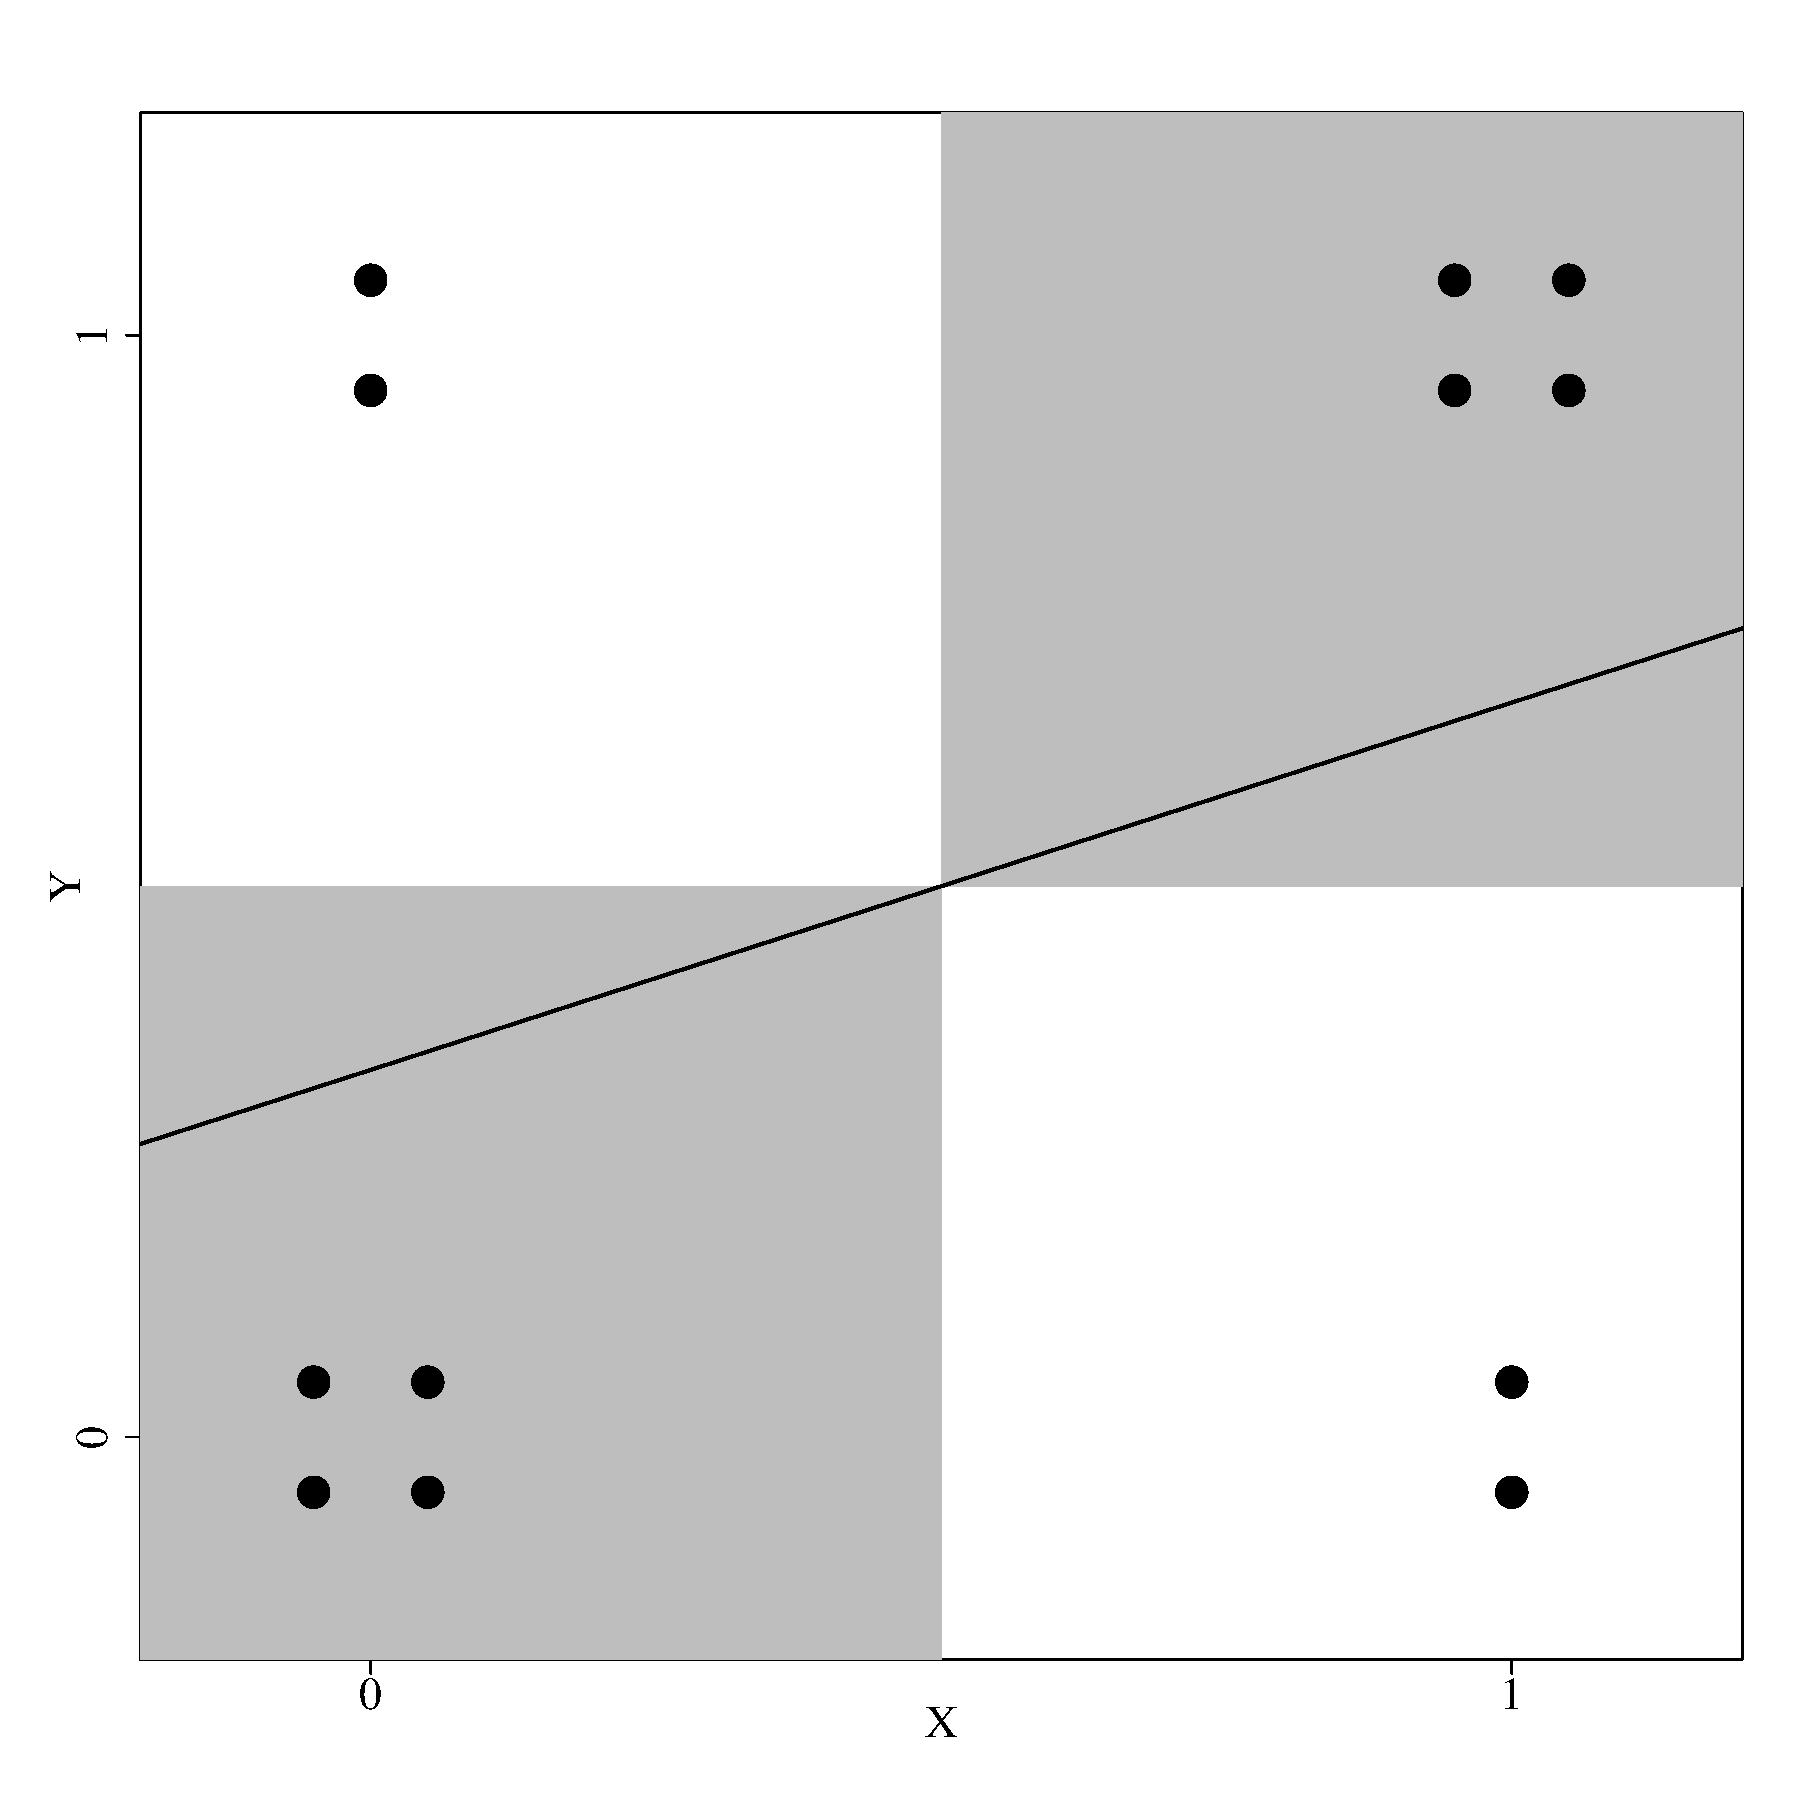
\includegraphics[width=3in]{BoundRegMatchPosA.pdf}
\end{figure}

}

\frame{
\frametitle{Introductory Exercise}

\begin{figure}[ht] \centering
        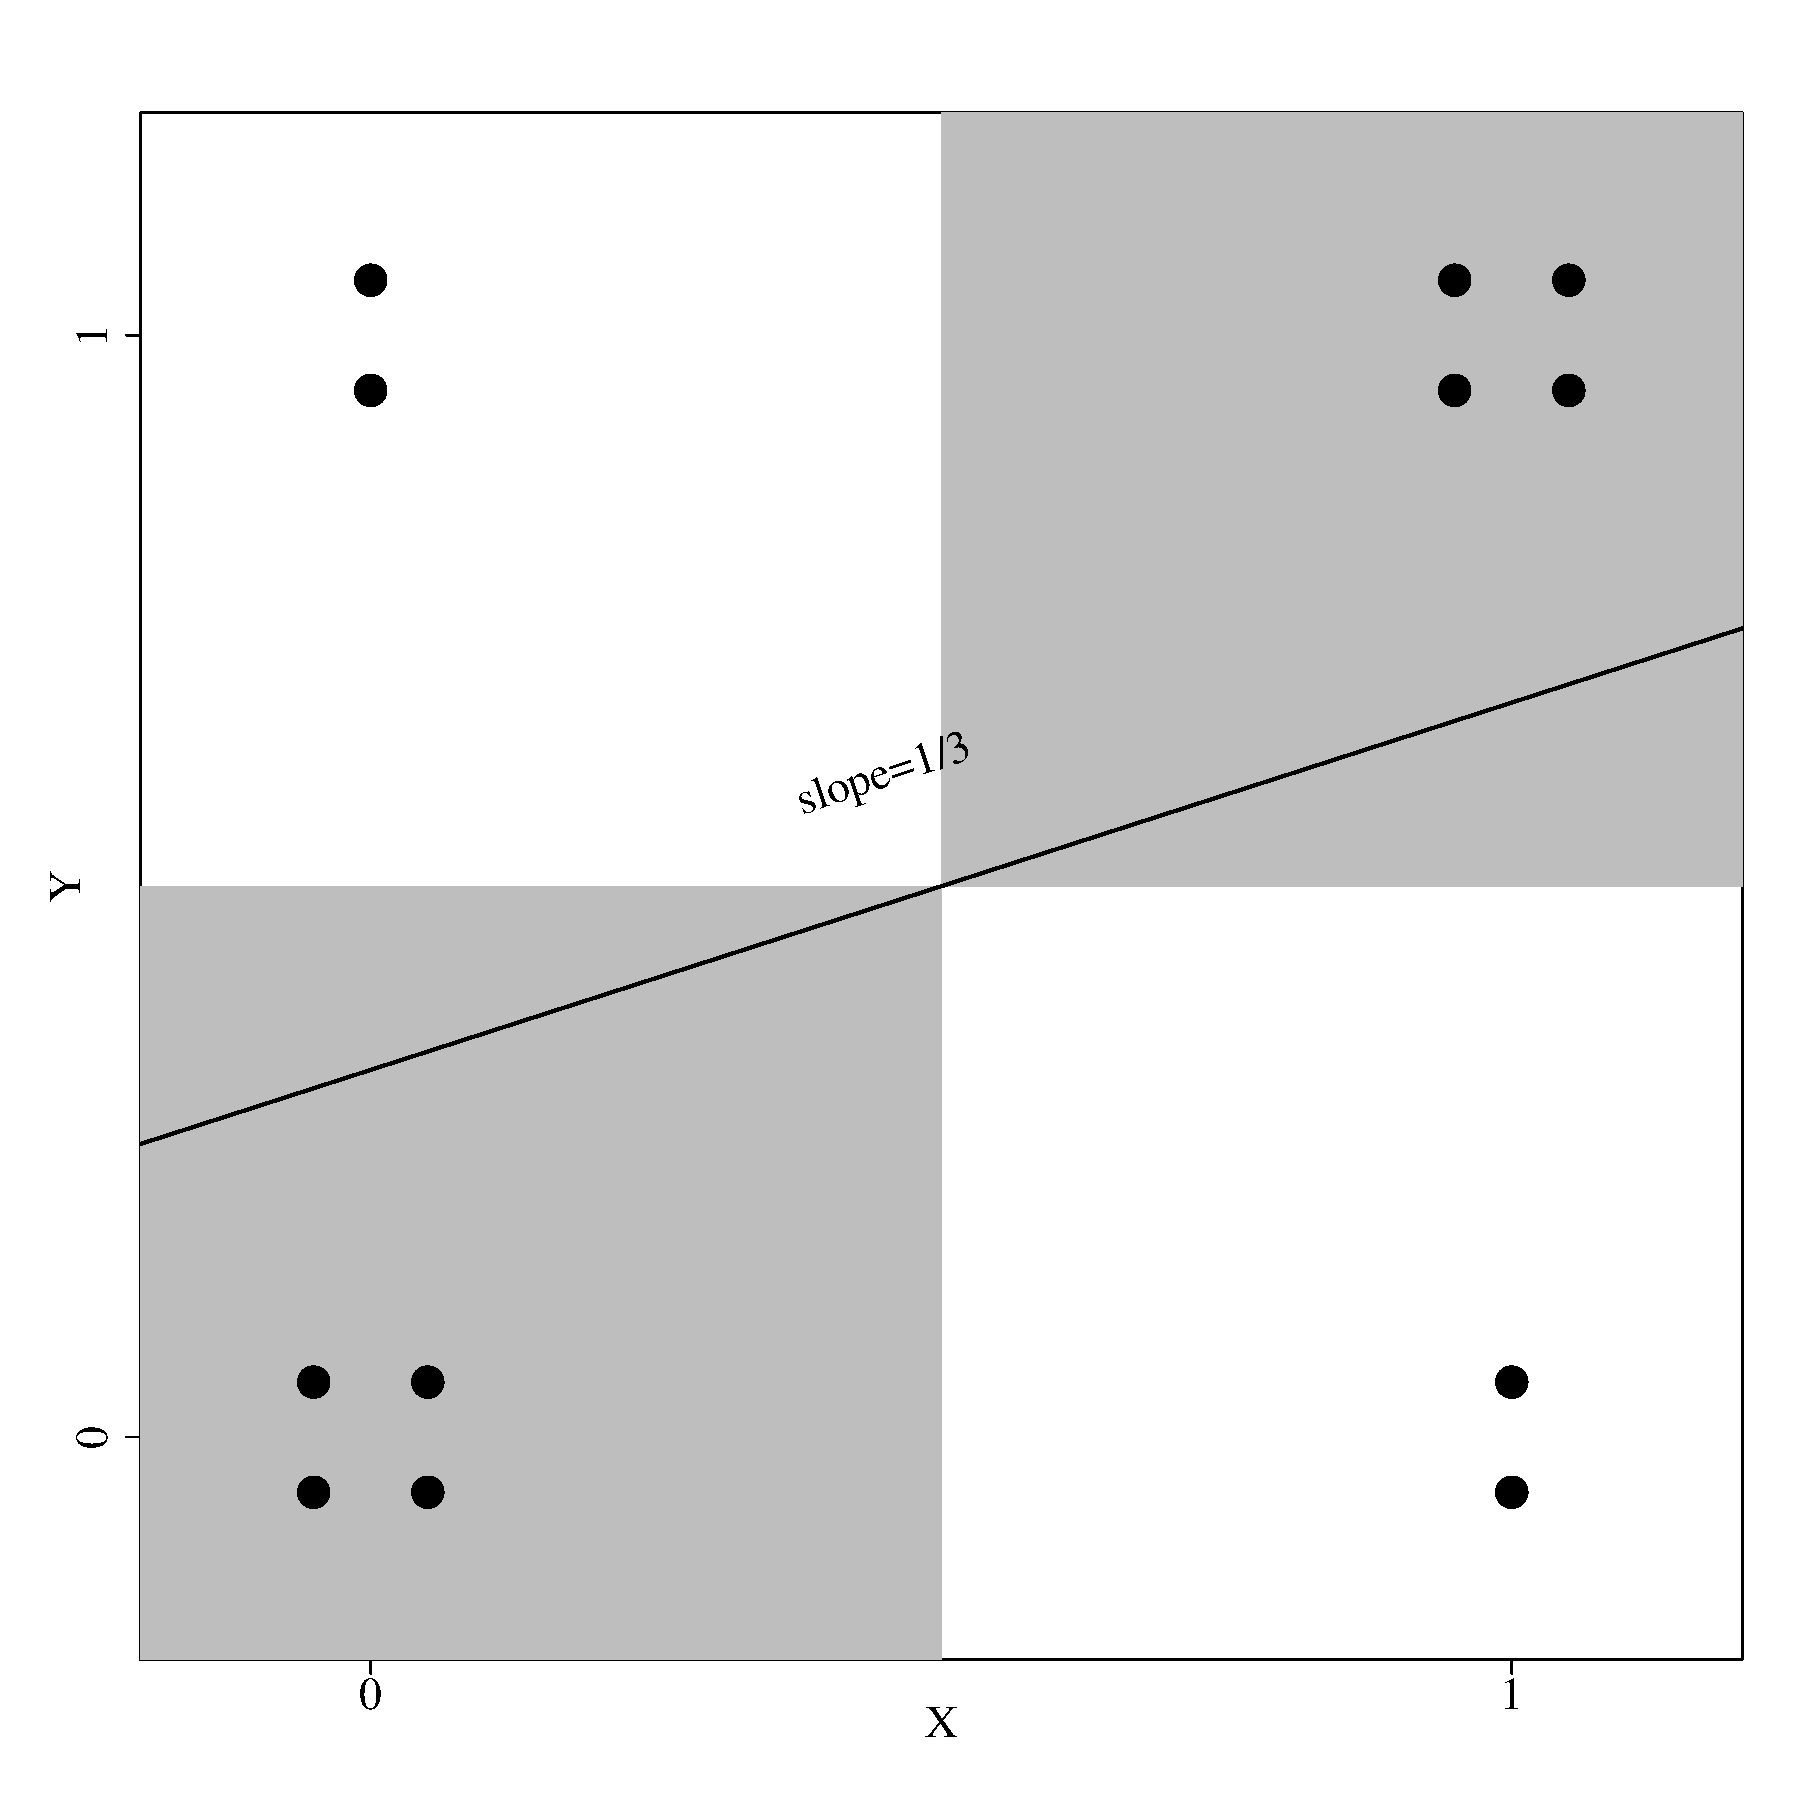
\includegraphics[width=3in]{BoundRegMatchPosB.pdf}
\end{figure}

}

\frame{
\frametitle{Introductory Exercise}

\begin{figure}[ht] \centering
        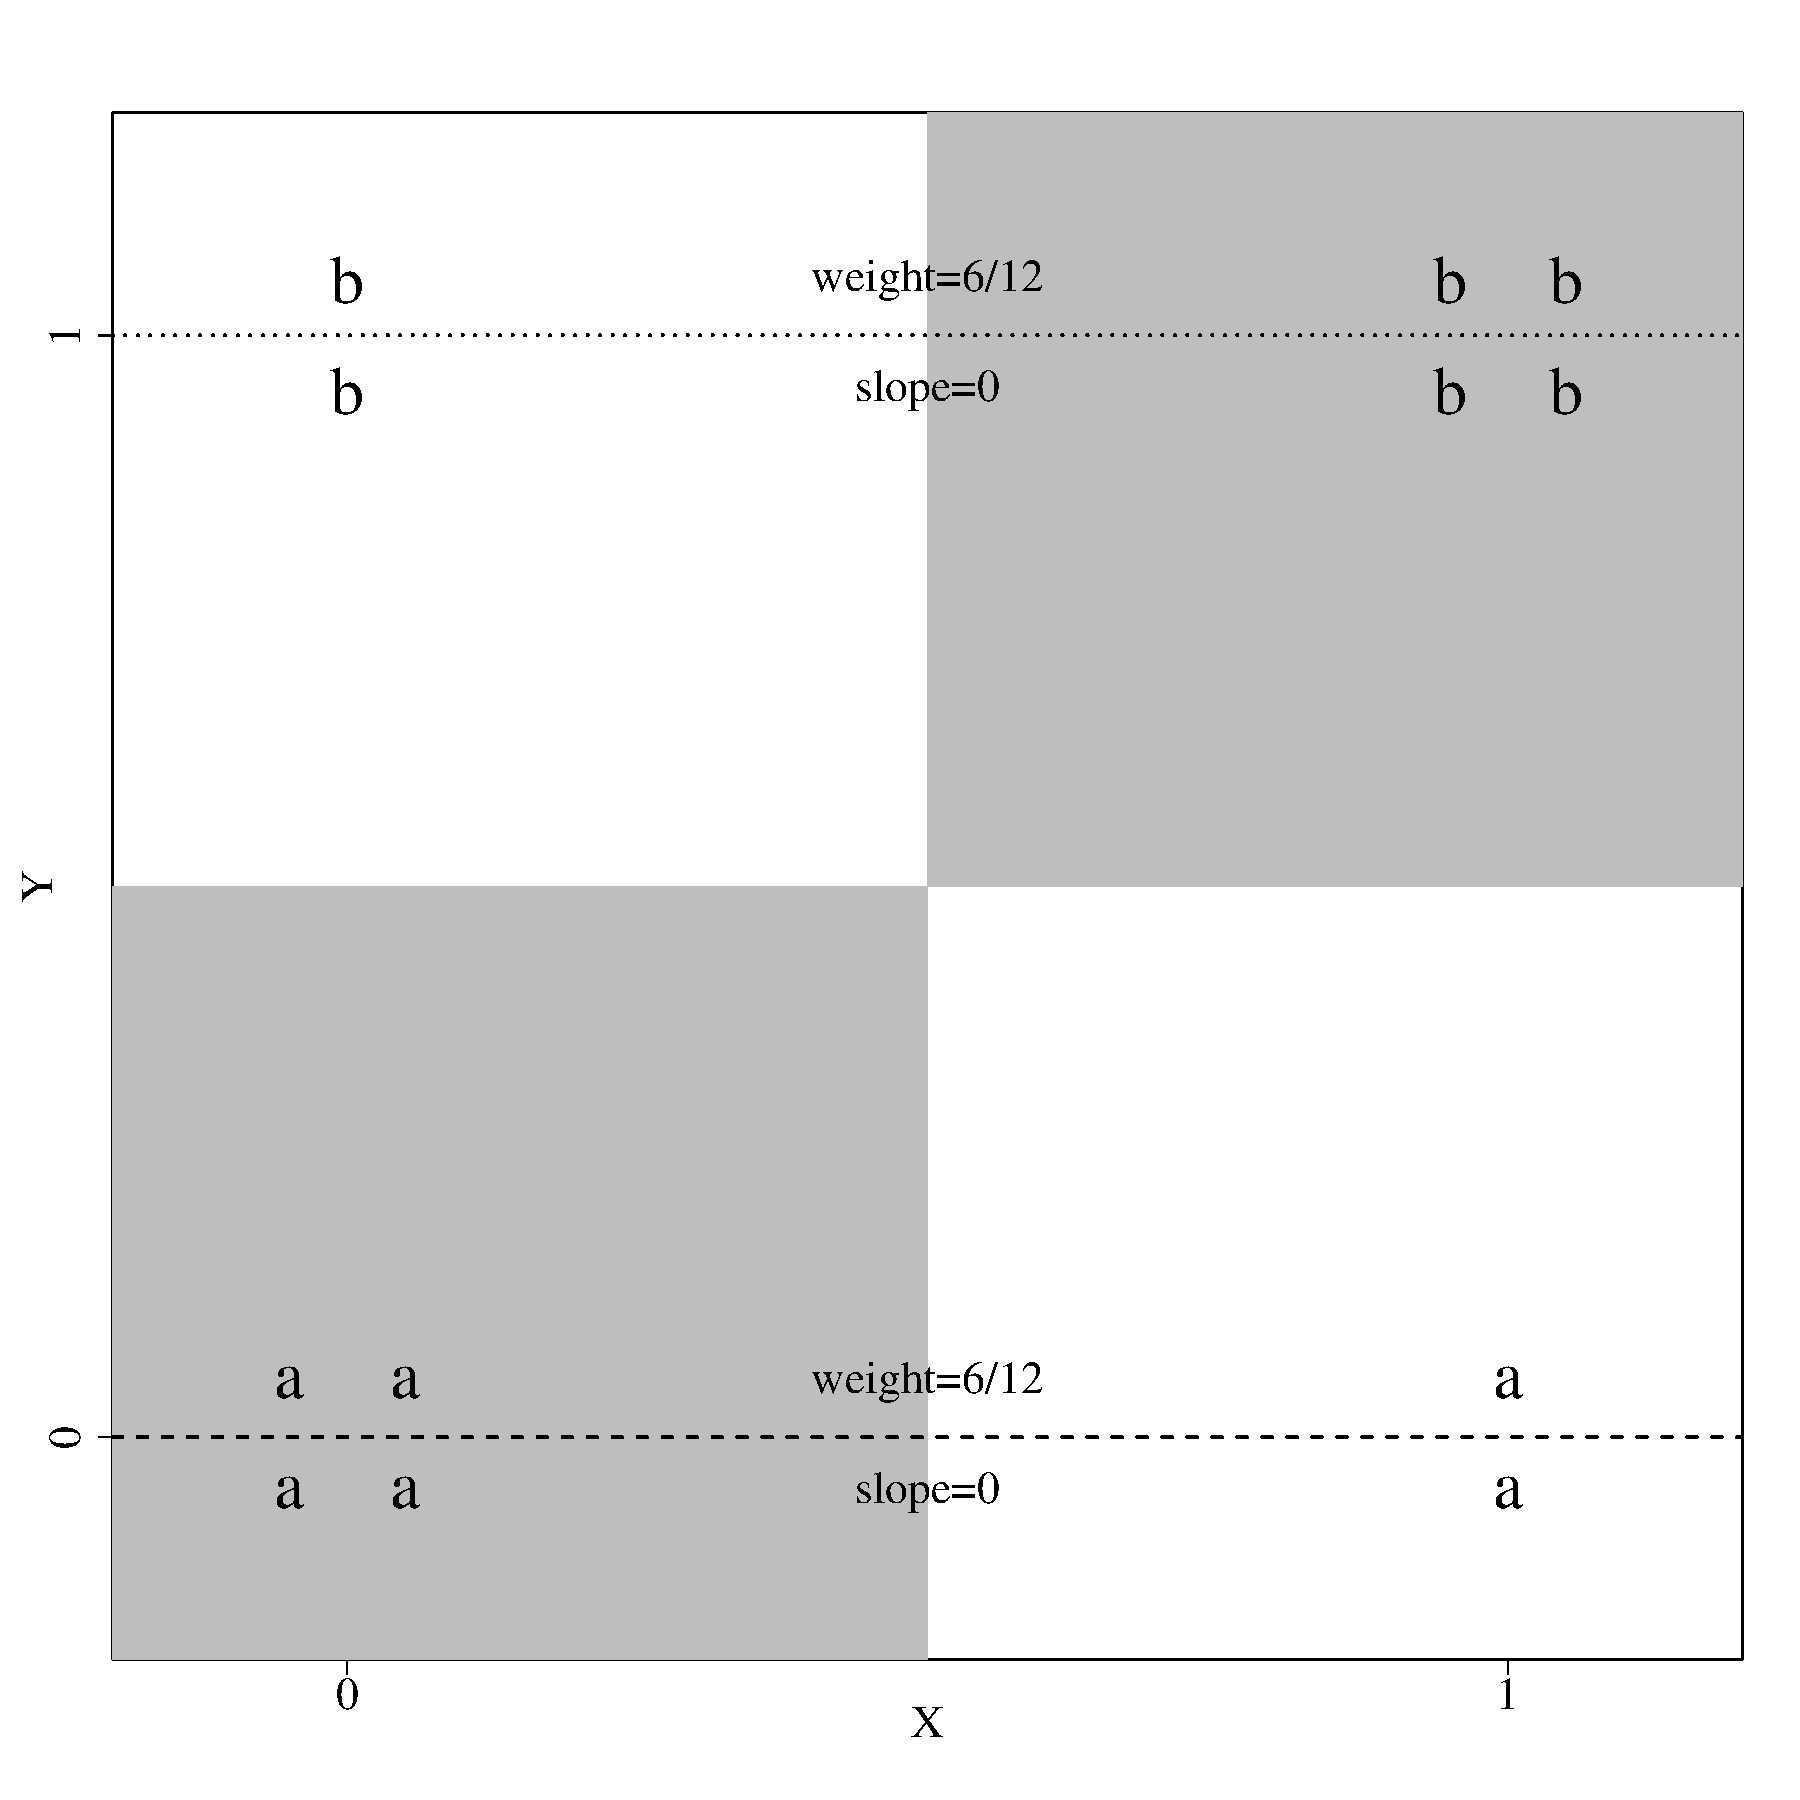
\includegraphics[width=3in]{BoundRegMatchZero.pdf}
\end{figure}

}

\frame{
\frametitle{Introductory Exercise}

\begin{figure}[ht] \centering
        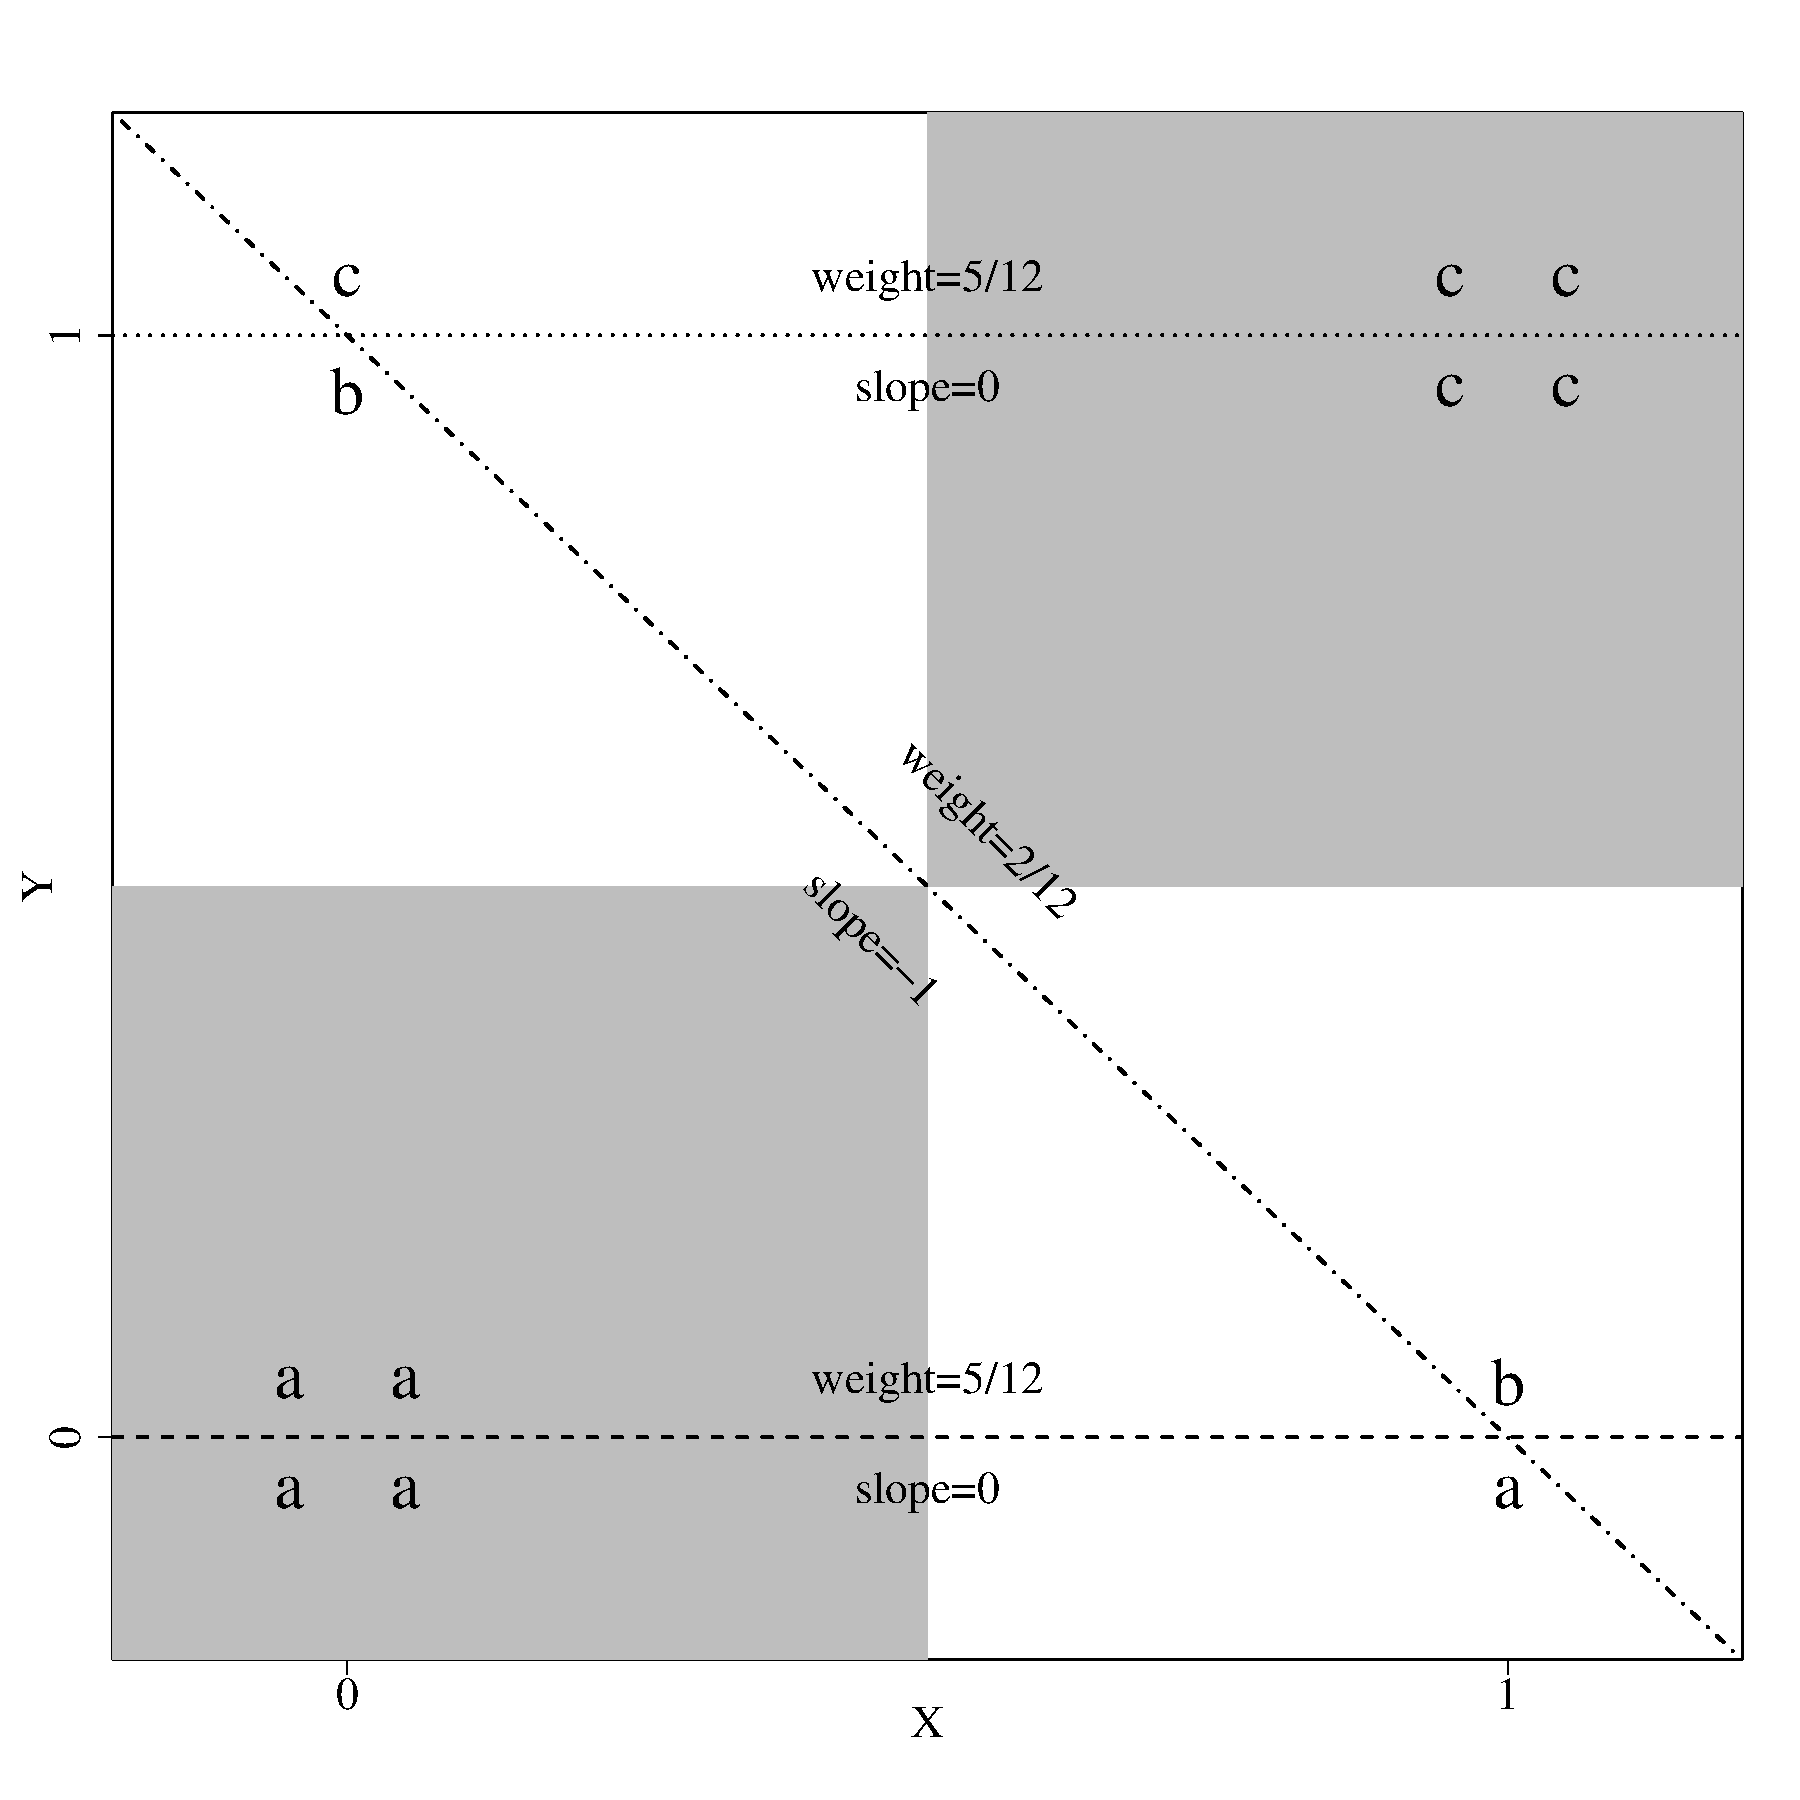
\includegraphics[width=3in]{BoundRegMatchNeg.pdf}
\end{figure}

}

\frame{
\frametitle{Introductory Exercise}

\begin{figure}[ht] \centering
        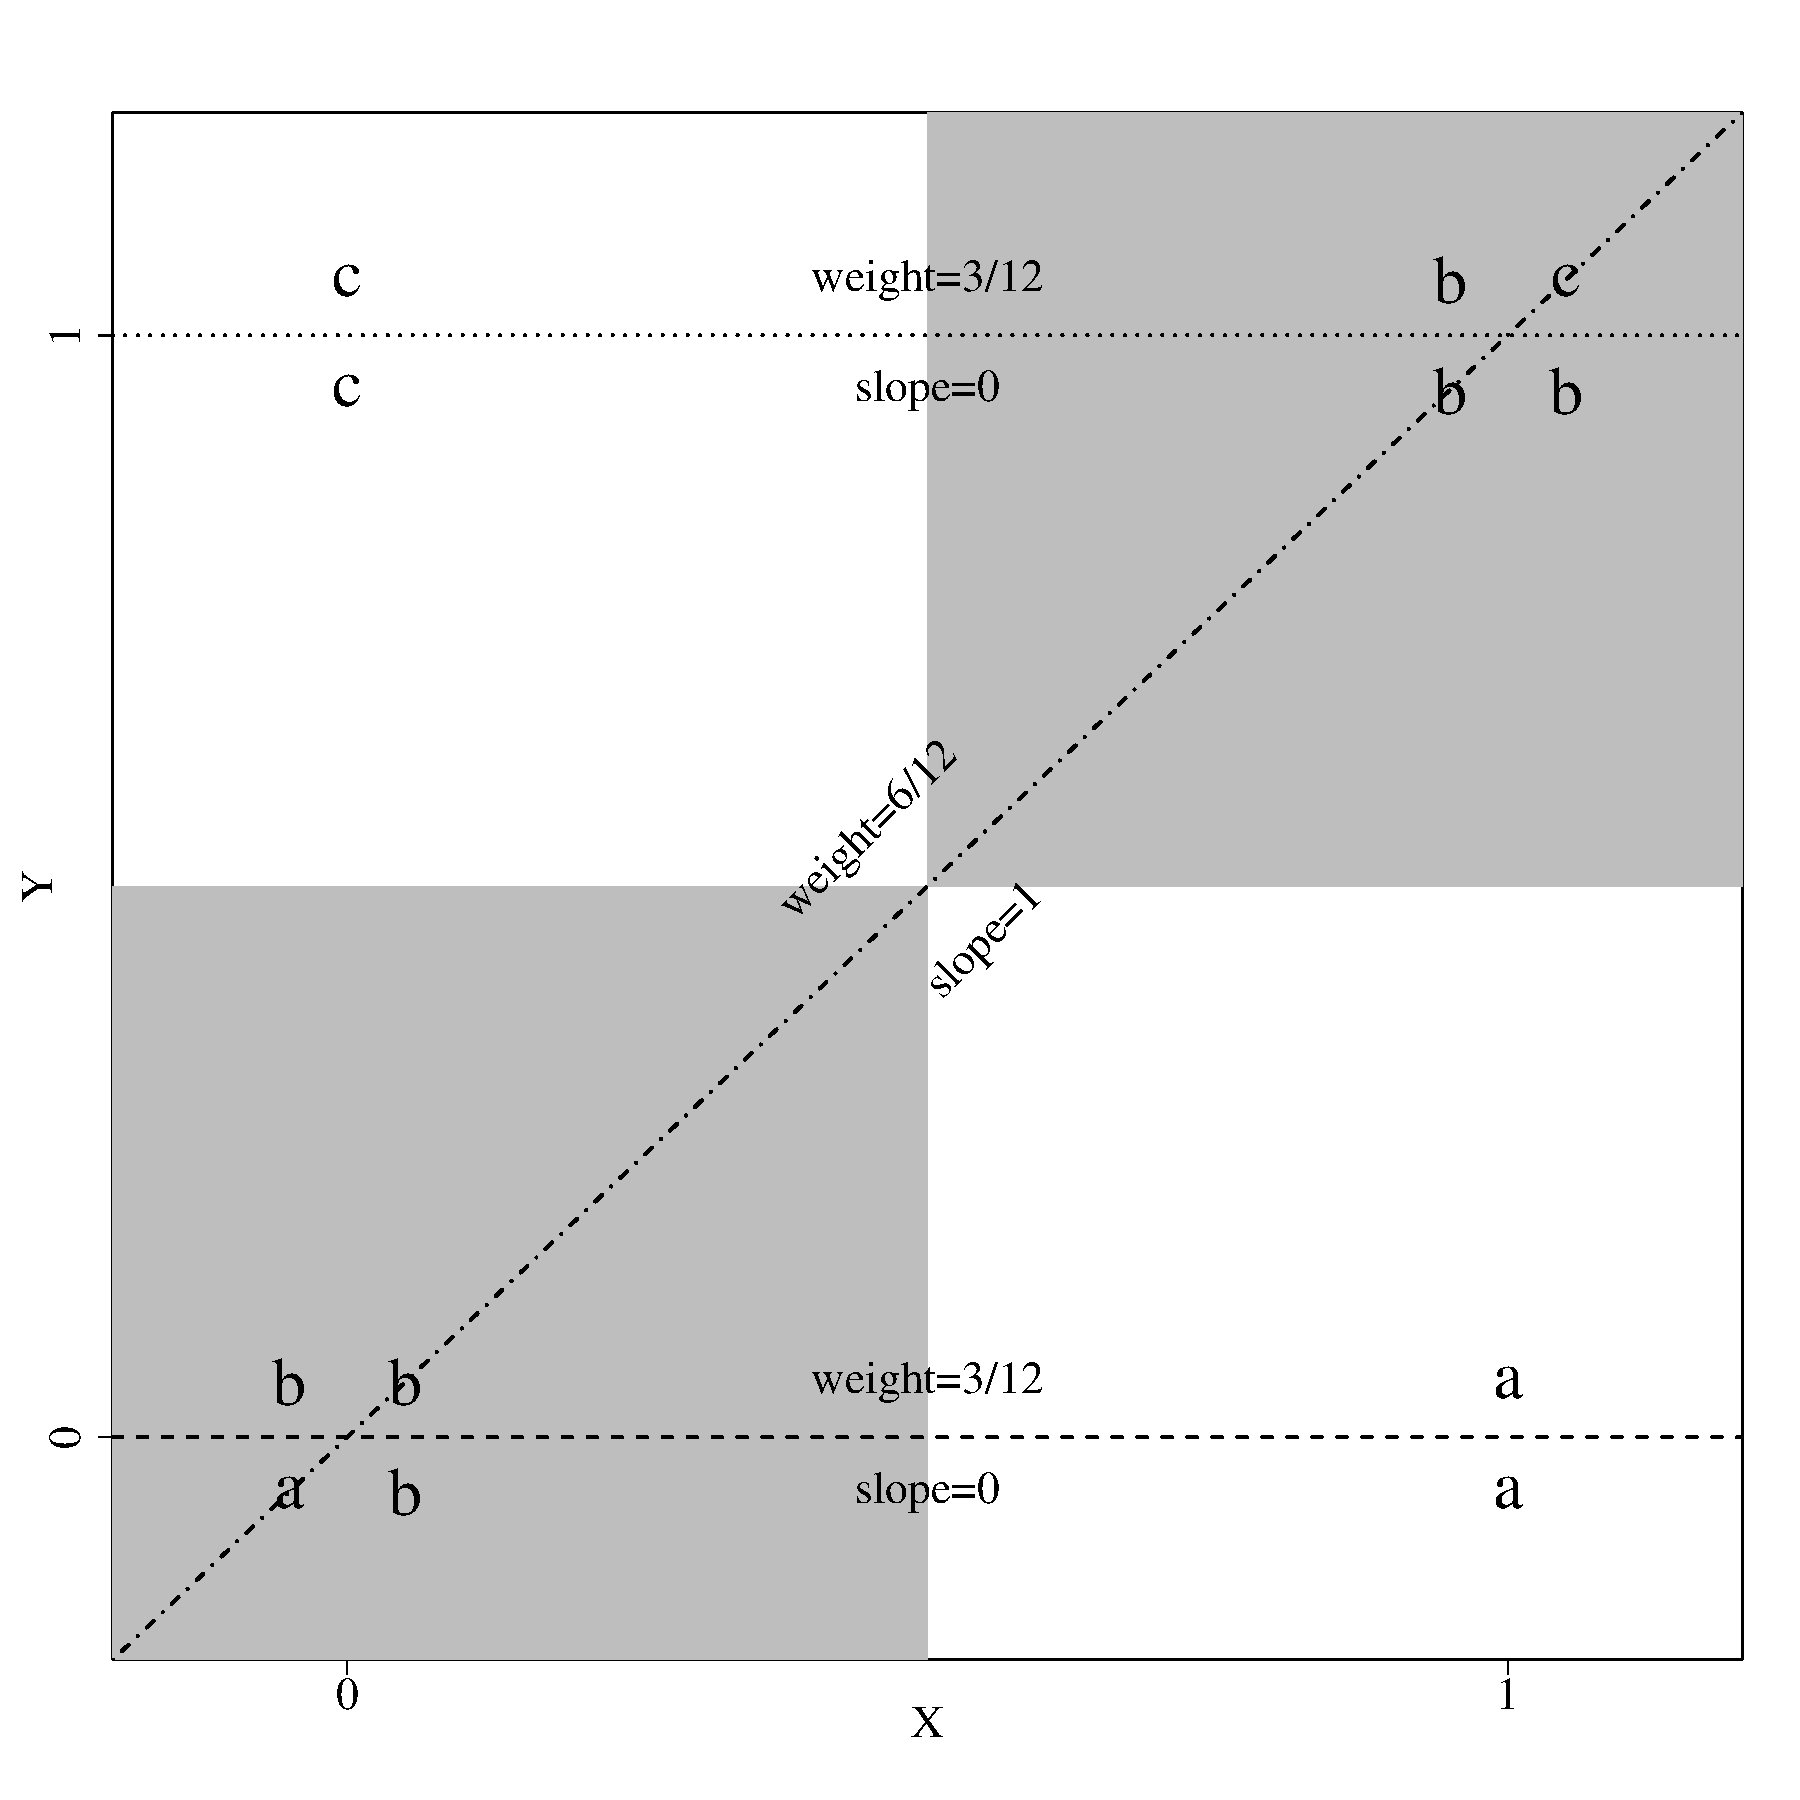
\includegraphics[width=3in]{BoundRegMatchBigPos.pdf}
\end{figure}

}


\section{Additive Multiple Linear Regression}


\frame{
\frametitle{More Than One Conditioning Variable}

\begin{itemize}
\item Often we want averages conditional on more than one variable.
\item As with continuous conditioning variables, there are many ways to do this.
\item Today we will look at two commonly used ``linear'' versions.
\item Unless the two conditioning variables are binary and an interaction is included, these approaches will induce misspecification.
\end{itemize}


}

\frame{
\frametitle{Multiple Regression with 2 Conditioning Variables}

\begin{itemize}
\item Fitted Values from the LCMF $\hat{y}_i = B_0 + B_1 x_i + B_2 z_i$\\
 for $i=1,...,N$ \pause
\item Residuals from Fitted Values:  $e_i = y_i - \hat{y}_i$ for $i=1,...,N$
\end{itemize} \pause

\vspace{.5cm}

Again, we choose $B_0$, $B_1$, and $B_2$, to minimize the SSR, where
\begin{align*}
SSR &= \sum_{i=1}^N e_i^2
\end{align*}
but the definition of $e_i$ changes with the inclusion of more variables. 
}
\frame{
\frametitle{One Binary and One Continuous Conditioning Variable}

\begin{figure}[ht] \centering
        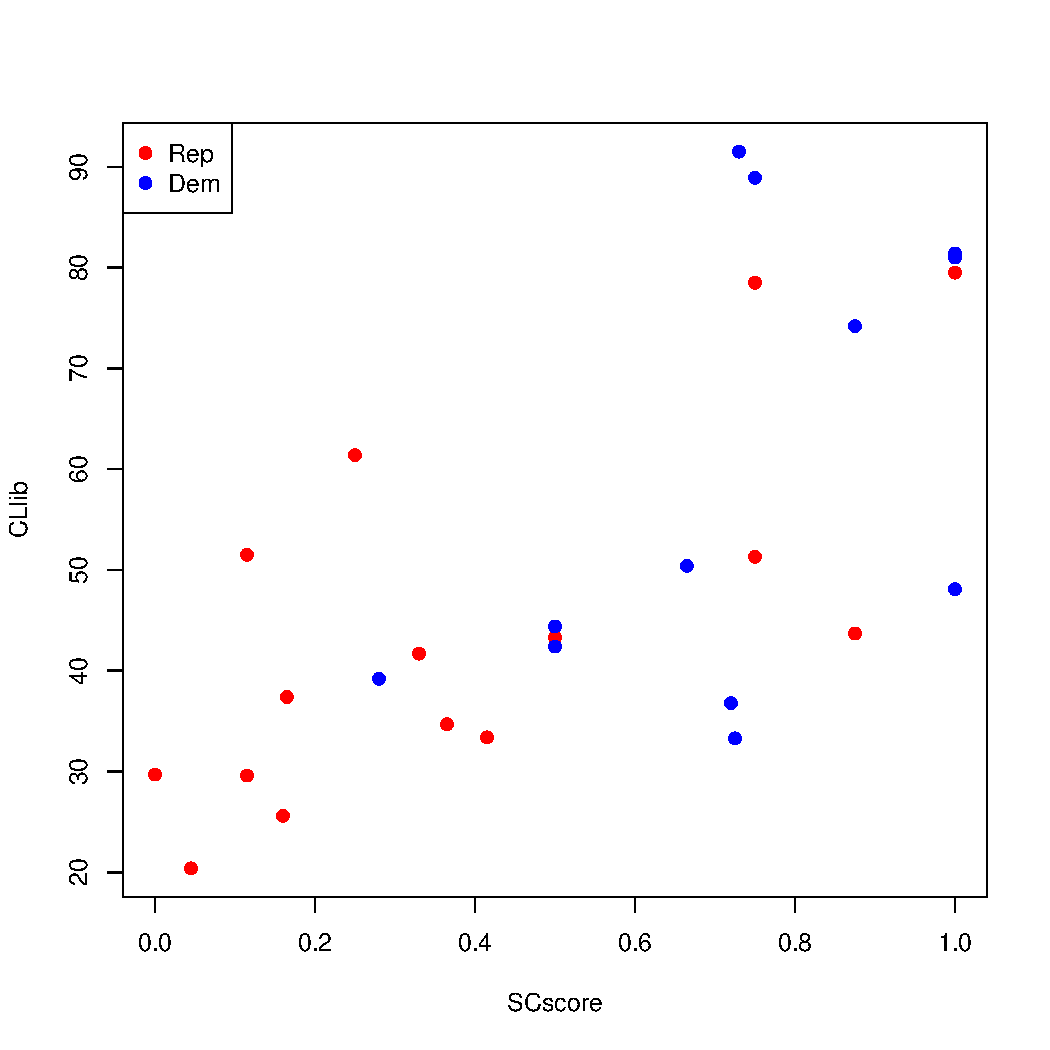
\includegraphics[width=3in]{psc.pdf}
\end{figure}

}

\frame{
\frametitle{One Binary and One Continuous Conditioning Variable}

\begin{figure}[ht] \centering
        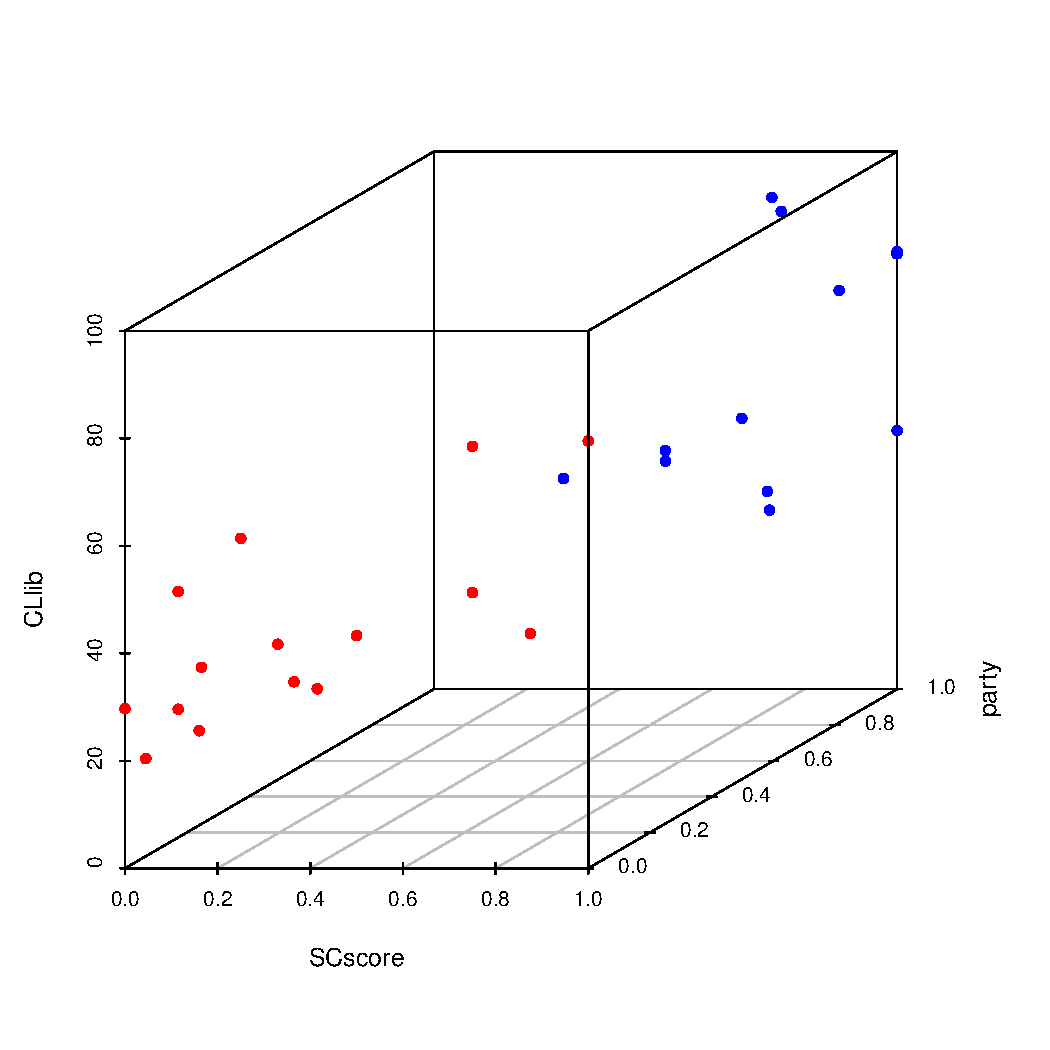
\includegraphics[width=3in]{em3D1.pdf}
\end{figure}
}

\frame{
\frametitle{One Binary and One Continuous Conditioning Variable}

\begin{figure}[ht] \centering
        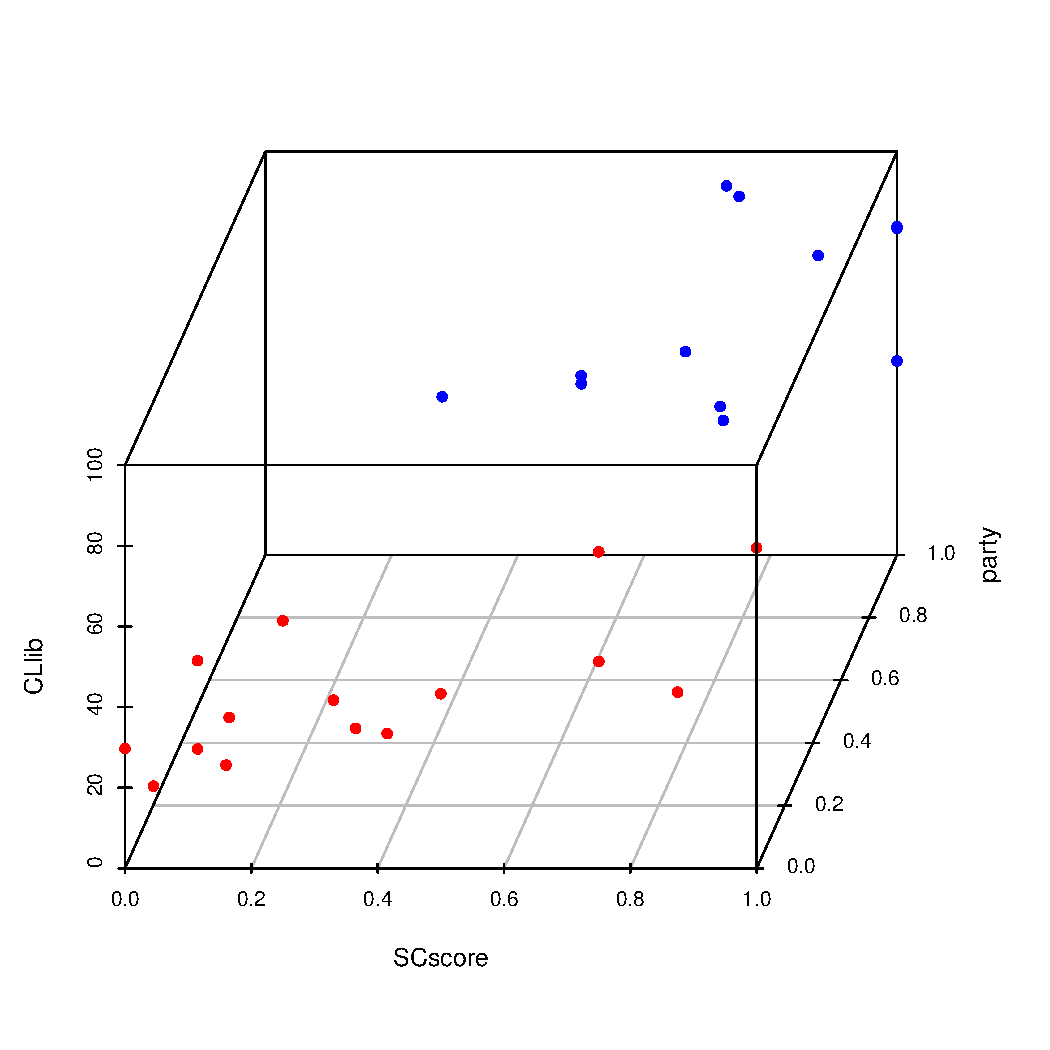
\includegraphics[width=3in]{em3D2.pdf}
\end{figure}
}

\frame{
\frametitle{Regression Plane}
\begin{figure}[ht] \centering
        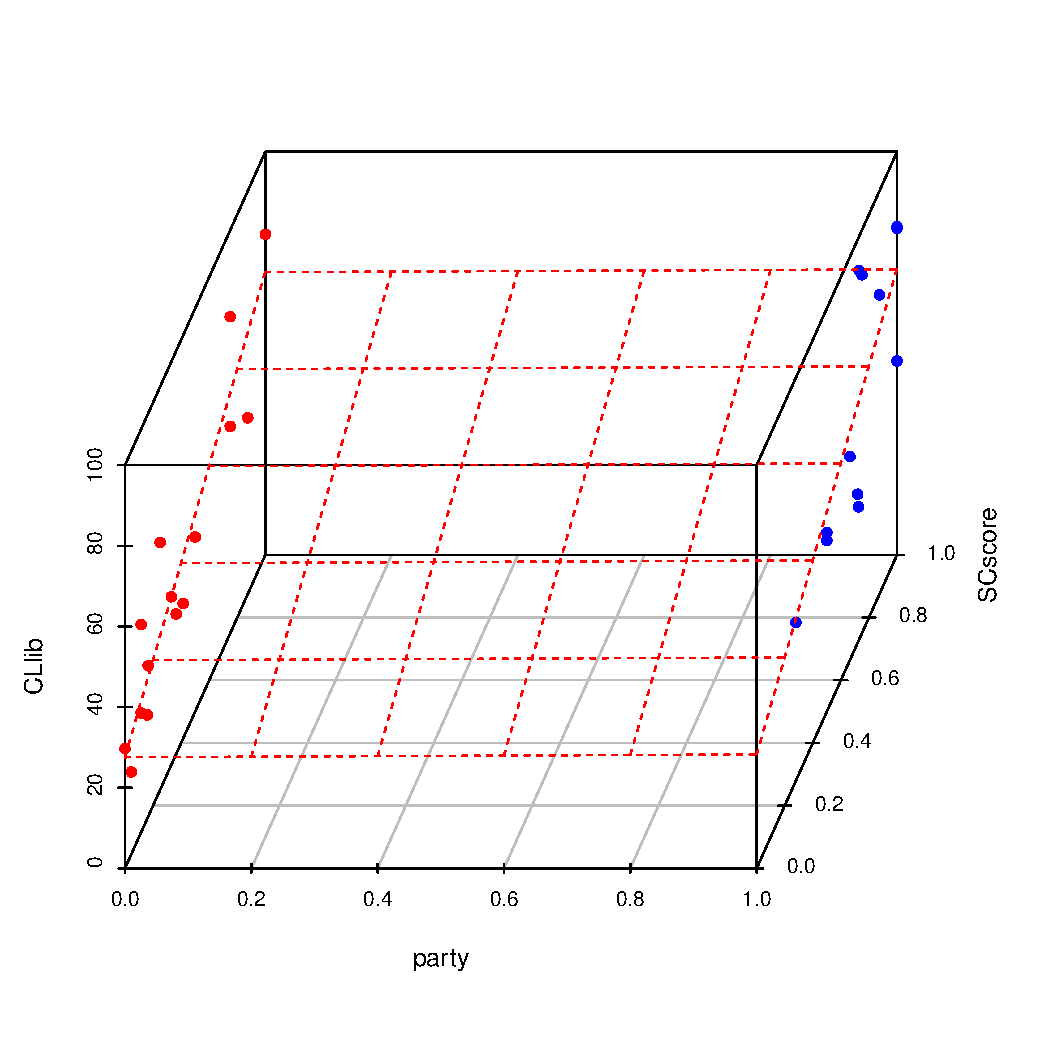
\includegraphics[width=3in]{em3D3.pdf}
\end{figure}
}

\frame{
\frametitle{Misspecification Activity}
Draw the two regression lines (i.e., edges of the regression plane) implied by 
$$
\hat{y} = B_0 + B_1 x + B_2 z
$$
\begin{figure}[ht] \centering
        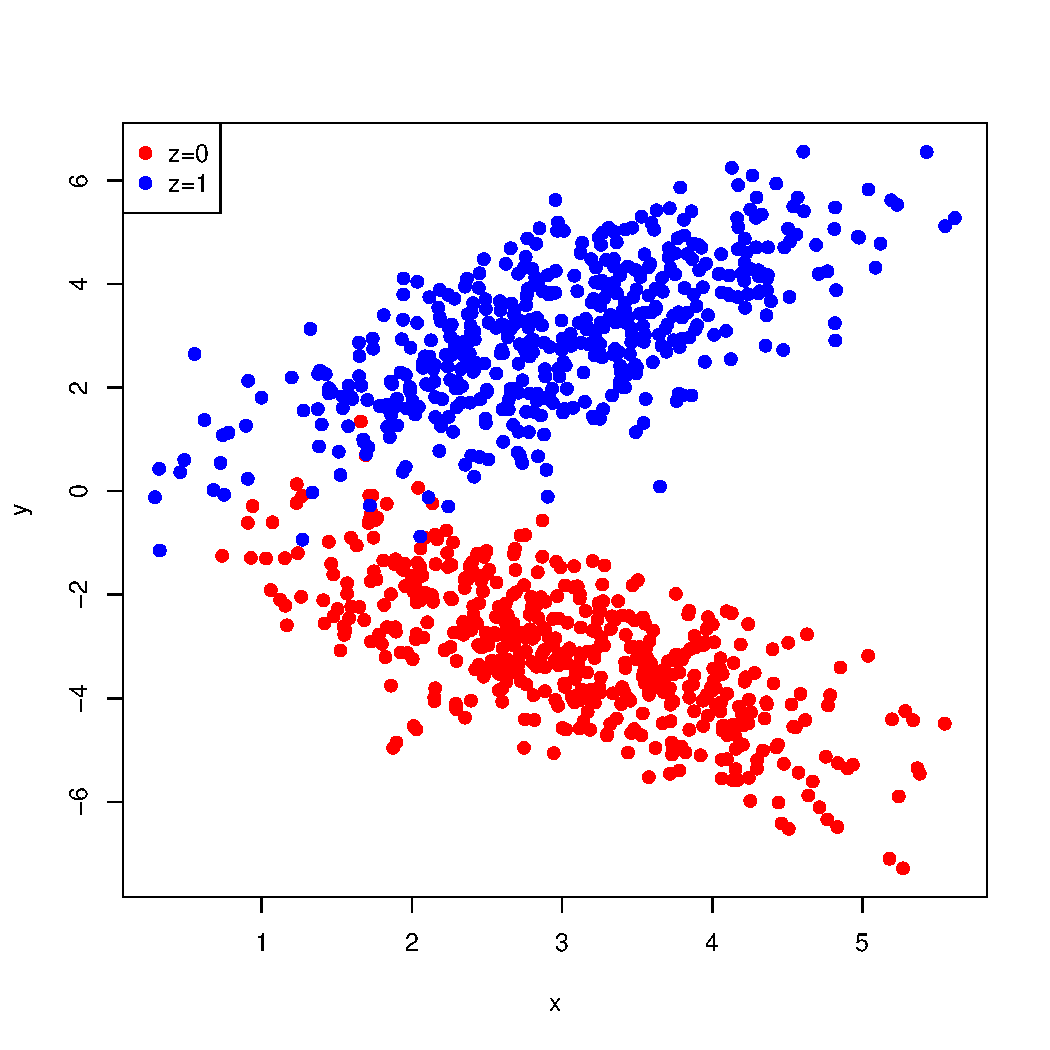
\includegraphics[width=2.5in]{multAct.pdf}
\end{figure}

}

\frame{
\frametitle{Misspecification  Activity}
Draw the two regression lines (i.e., edges of the regression plane) implied by 
$$
\hat{y} = B_0 + B_1 x + B_2 z
$$
\begin{figure}[ht] \centering
        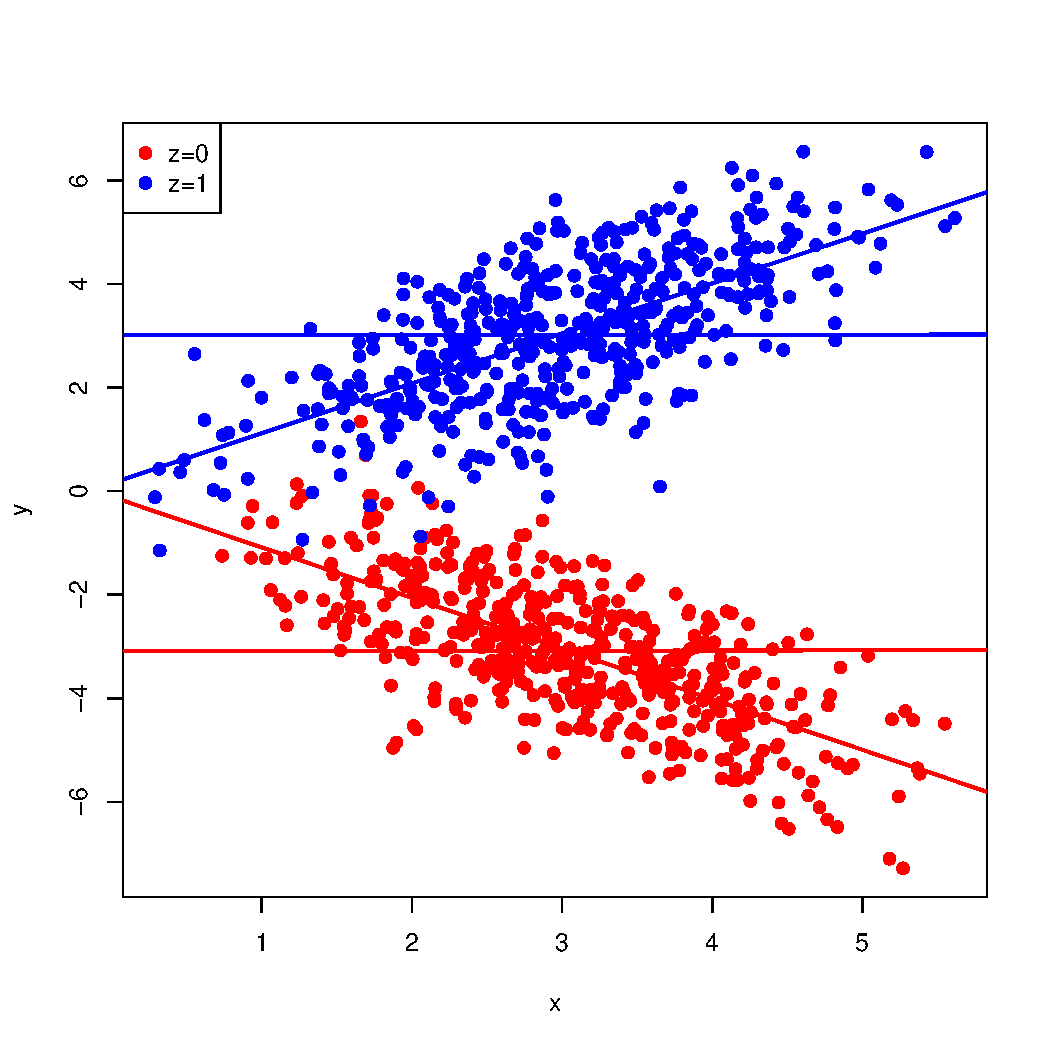
\includegraphics[width=2.5in]{multActSol.pdf}
\end{figure}

}


\frame{
\frametitle{Regression Plane for Two Continuous Conditioning Variables}

\begin{figure}[ht] \centering
        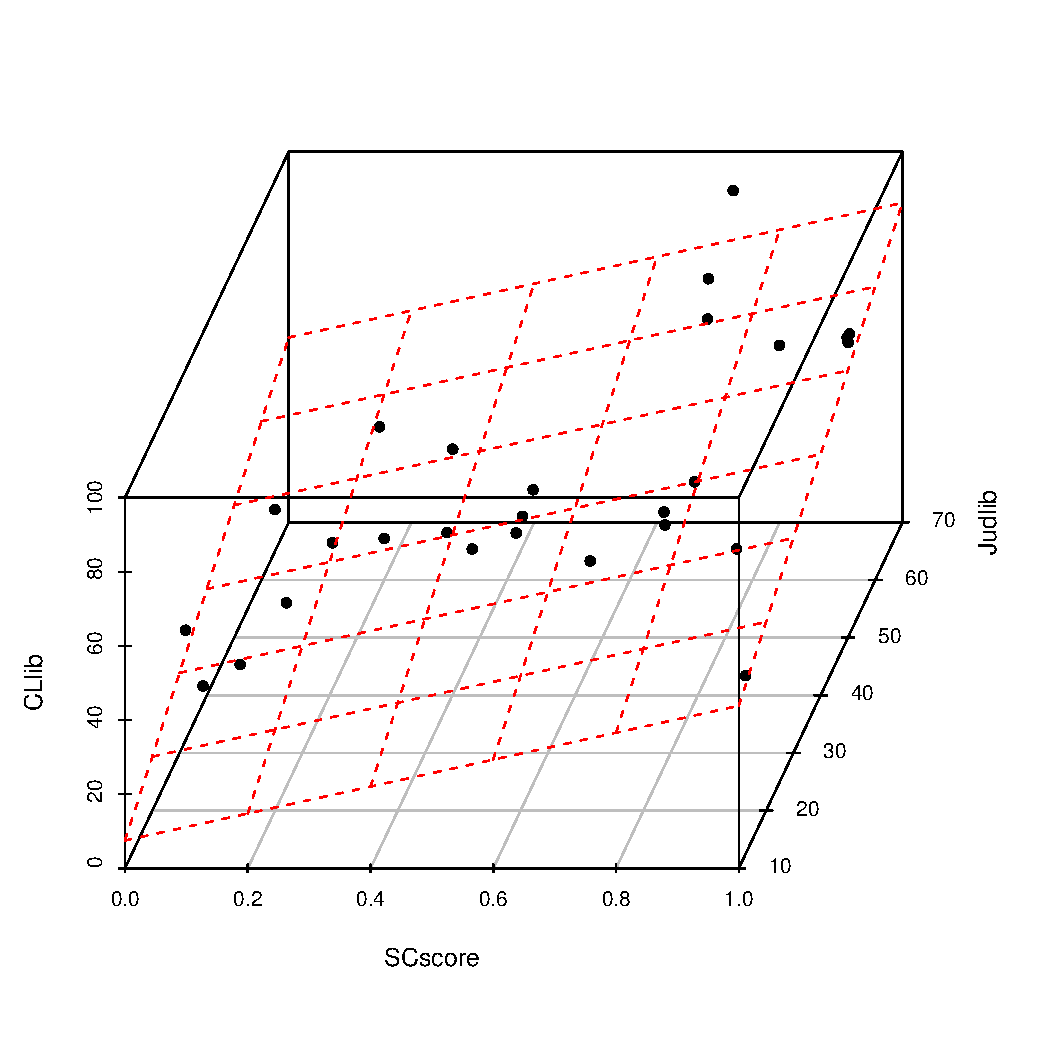
\includegraphics[width=3in]{em3D4.pdf}
\end{figure}
}


\frame{
\frametitle{Descriptive Interpretation of Additive Regression}

$$\widehat{CLlib}_i = B_0 + B_1 \cdot SCscore_i + B_2 \cdot Dem_i$$

\begin{figure}[ht] \centering
        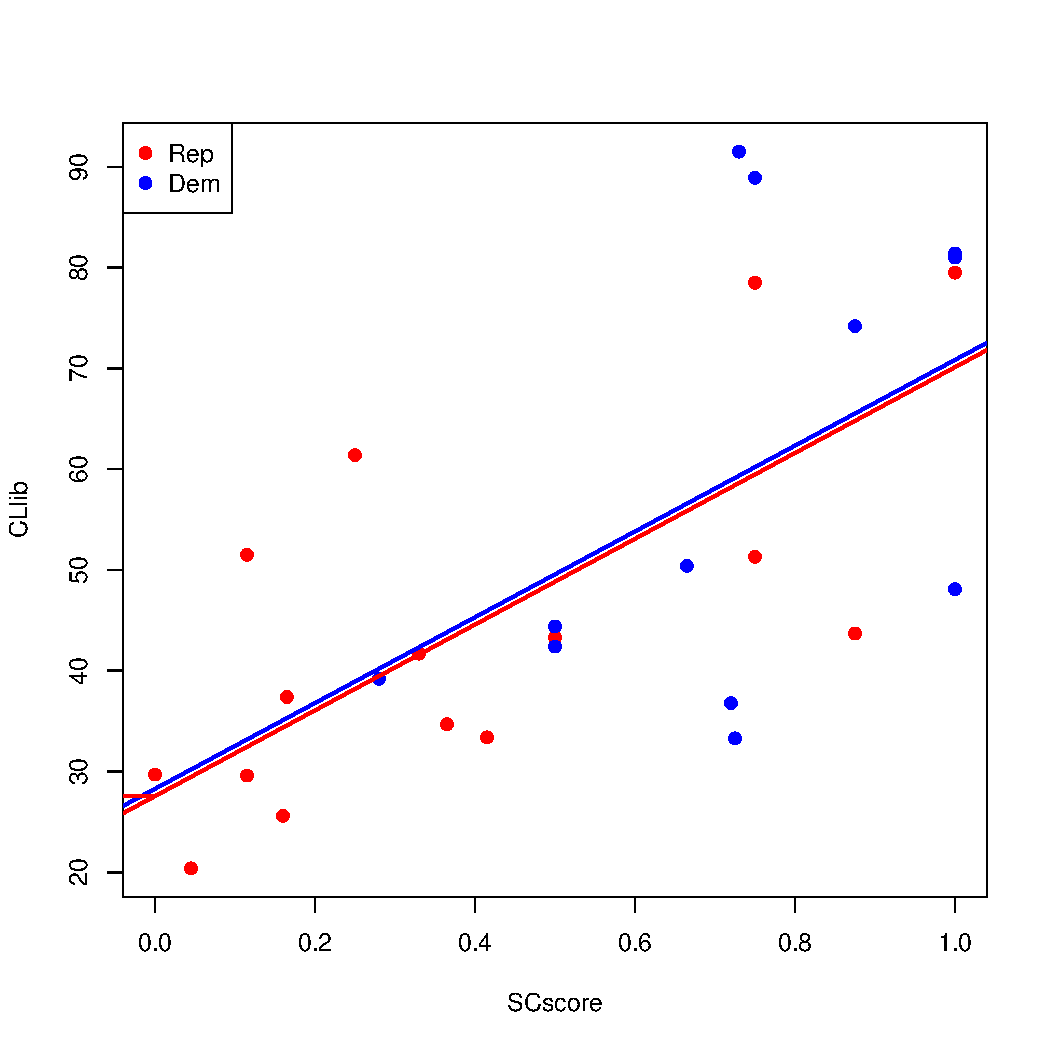
\includegraphics[width=2.7in]{pscMarg.pdf}
\end{figure}

}

\frame{
\frametitle{Recall: Simple Regression with SCscore}

$$\widehat{CLlib}_i = B_0 + B_1 \cdot SCscore_i $$

\begin{figure}[ht] \centering
        \scalebox{.4}{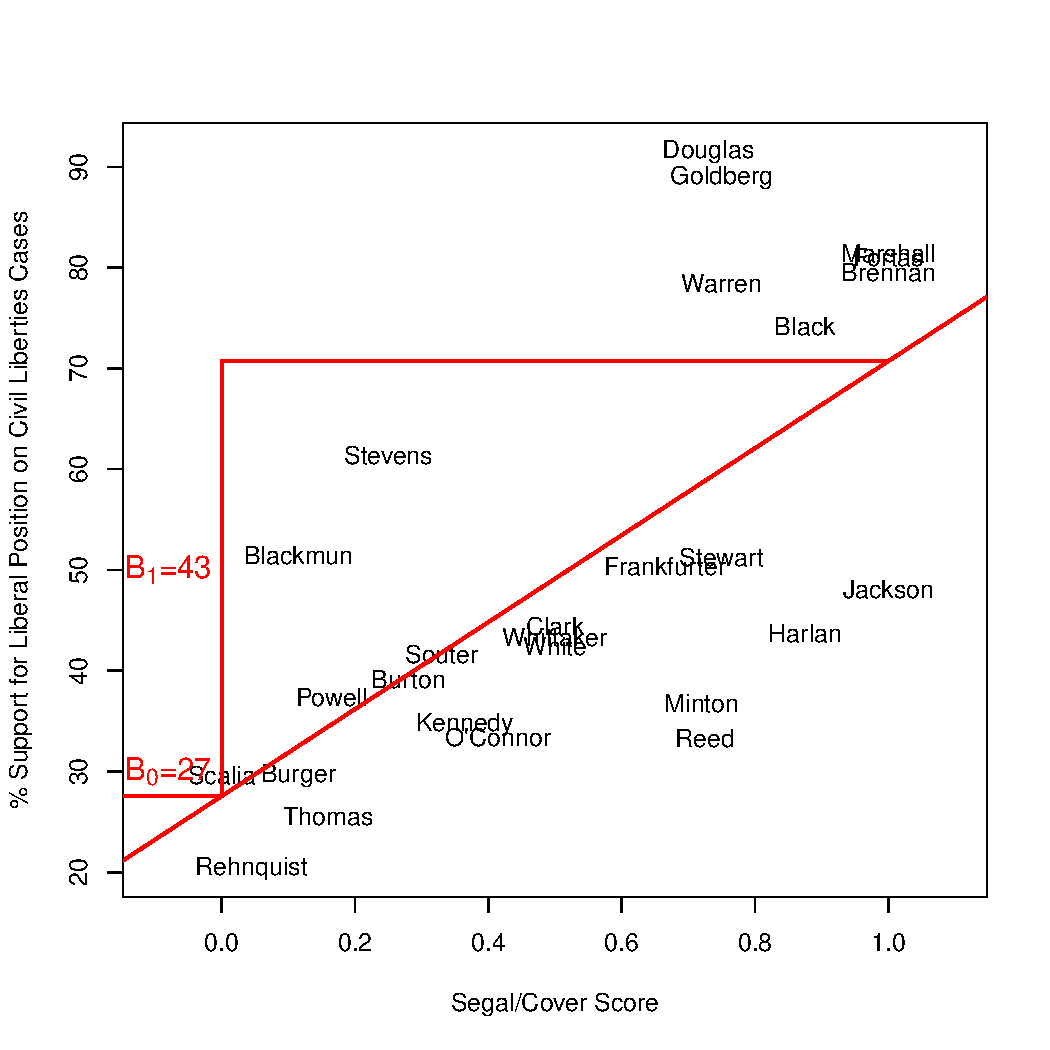
\includegraphics{lmPlot.pdf}}
\end{figure}

}

\frame{
\frametitle{Recall: Simple Regression with Party}

$$\widehat{CLlib}_i = B_0 + B_1 \cdot Dem_i$$

\begin{figure}[ht] \centering
        \scalebox{.4}{
\includegraphics{lmBin.pdf}}
\end{figure}


}

\frame{
\frametitle{Descriptive Interpretation of Additive Regression}

$$\widehat{CLlib}_i = B_0 + B_1 \cdot SCscore_i + B_2 \cdot Dem_i$$

\begin{figure}[ht] \centering
        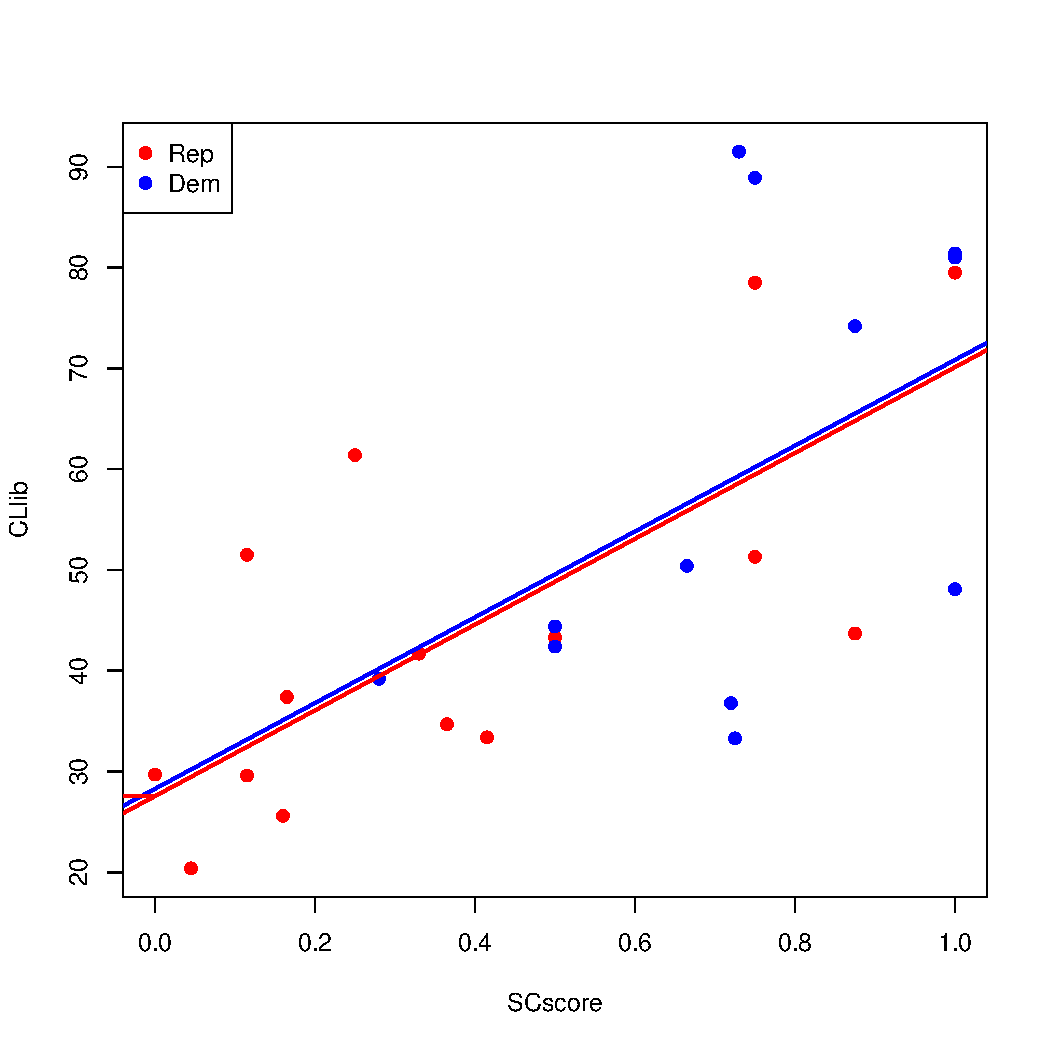
\includegraphics[width=2.7in]{pscMarg.pdf}
\end{figure}

}



\frame{
\frametitle{Descriptive Interpretation of Additive Regression}

$$\widehat{Fedlib}_i = B_0 + B_1 \cdot SCscore_i + B_2 \cdot Dem_i$$

\begin{figure}[ht] \centering
      \includegraphics<1>[width=2.7in]{pscMarg2.pdf}
	\includegraphics<2>[width=2.7in]{pscMarg20.pdf}
	\includegraphics<3>[width=2.7in]{pscMarg21.pdf}
	\includegraphics<4>[width=2.7in]{pscMarg22.pdf}
	\end{figure}

}

\frame{
\frametitle{Additive Interpretations}

\begin{itemize}
\item $B_0$: Mean outcome for a Rep justice with a zero SCscore.
\item $B_1$: Mean difference in outcomes between justices appointed by the same party, but with a one unit difference in SCscore.
\item $B_2$: Mean difference in outcomes between justices with the same SCscore, but appointed by different parties (Dem minus Rep).
\end{itemize}
\bigskip

Discuss the additive linear model assumptions implicit in these interpretations. 

}


%\frame{
%\frametitle{Two reasons slope doesn't change}
%
%There are two reasons a slope doesn't change when including an additional variable in a regression
%
%\begin{itemize}
%\item if the original and additional control variables are uncorrelated
%\item if the slope for the additional variable in the multiple regression is zero
%\end{itemize}
%
%
%}

\section{Interactive Multiple Linear Regression}


\frame{
\frametitle{Multiple Regression with an Interaction}

\begin{itemize}
\item Fitted Values: $\hat{y}_i = B_0 + B_1 x_i + B_2 z_i + B_3 x_i \cdot z_i$ \\
for $i=1,...,N$ \pause
\item Residuals:  $e_i = y_i - \hat{y}_i$ for $i=1,...,N$
\end{itemize} \pause

\vspace{.5cm}

Again, we choose $B_0$, $B_1$, $B_2$, and $B_3$, to minimize the SSR, where
\begin{align*}
SSR &= \sum_{i=1}^N e_i^2
\end{align*}
but the definition of $e_i$ has again changed. 
}




\frame{
\frametitle{Descriptive Interpretation of Interaction Model}

$$\widehat{Fedlib}_i = B_0 + B_1 \cdot SCscore_i + B_2 \cdot Dem_i + B_3 \cdot SCscore_i \cdot Dem_i$$

\begin{figure}[ht] \centering
      \includegraphics<1>[width=2.7in]{pscInt.pdf}
	\includegraphics<2>[width=2.7in]{pscInt0.pdf}
	\includegraphics<3>[width=2.7in]{pscInt1.pdf}
	\includegraphics<4>[width=2.7in]{pscInt2.pdf}
	\includegraphics<5>[width=2.7in]{pscInt3.pdf}

\end{figure}

}

\frame{
\frametitle{Interactive Interpretations}

\begin{itemize}
\item $B_0$: Mean outcome for a Rep justice with a zero SCscore.
\item $B_1$: Mean difference in outcomes between justices appointed by Republicans, but with a one unit difference in SCscore.
\item $B_0 + B_2$:  Mean outcome for a Dem justice with a zero SCscore.
\item $B_2$: Mean difference in outcomes between justices with a zero SCscore, but appointed by different parties (Dem minus Rep).
\item $B_1+ B_3$:  Mean difference in outcomes between Dem justices with a one unit difference in SCscore.
\item $B_3$: Mean difference between the mean difference in outcomes between Dem justices with a one unit difference in SCscore and the mean difference in outcomes between Rep justices with a one unit difference in SCscore.
\end{itemize}
}

\frame{
\frametitle{Variance and Multiple Regression}

\begin{itemize}
\item As before, we want to assess the ``leastness'' of  least squares (i.e., the spread of the data around the plane or twisted plane).
\item The standard error of the regression, $\sqrt{\frac{\sum_{i=1}^N e_i^2}{N-k}}$, now accounts for the number of $B$'s in the model (where $k$ is the number of $B$'s).
\item $R^2$ uses the same formula $1-\frac{SSR}{TSS}$, however the inclusion of additional variables will automatically reduce the SSR. 
\end{itemize}

}



\frame{
\frametitle{Summary Activity}

\begin{figure}[ht] \centering
      \includegraphics<1>[width=2.7in]{finalAct.pdf}
	\includegraphics<2>[width=2.7in]{finalAct1.pdf}
	\includegraphics<3>[width=2.7in]{finalAct2.pdf}
	\includegraphics<4>[width=2.7in]{finalAct3.pdf}
	\includegraphics<5>[width=2.7in]{finalAct4.pdf}
\end{figure}

}

\section{Adding/Removing Additive Variables}

\frame{
\frametitle{Multiple Regression with 2 Conditioning Variables}

\begin{itemize}
\item Fitted Values from the LCMF $\hat{y}_i = B_0 + B_1 x_i + B_2 z_i$\\
 for $i=1,...,N$ 
\item Residuals from Fitted Values:  $e_i = y_i - \hat{y}_i$ for $i=1,...,N$
\end{itemize}

\vspace{.5cm}

Again, we choose $B_0$, $B_1$, and $B_2$, to minimize the SSR, where
\begin{align*}
SSR &= \sum_{i=1}^N e_i^2 = \sum_{i=1}^N [y_i - (B_0 + B_1 x_i + B_2 z_i)]^2
\end{align*}
but the definition of $e_i$ changes with the inclusion of more variables. 
}

\frame{
\frametitle{Residuals and covariates uncorrelated}



\begin{align*}
\frac{\partial SSR}{\partial \tilde{B}_1} &=  - \sum_{i=1}^N 2e_i \cdot x_i \\
\frac{\partial SSR}{\partial \tilde{B}_2} &=  - \sum_{i=1}^N 2 e_i\cdot z_i
\end{align*}

\bigskip


We set both equal to zero when solving. 


}


\begin{frame}

Suppose we want $B_1$ from $y_i=B_{0}+B_{1}x_{i}+B_{2}z_{i}+e_i$, but we run the regression of $y$ on $x$ alone. Then,
{\small
\begin{align*}
&\frac{\sum\limits_{i=1}^{n}(x_i-\bar{x_{1}})y_{i}}{\sum\limits_{i=1}^{n}(x_i-\bar{x_{1}})^{2}}\\
&= \visible<2->{\frac{\sum\limits_{i=1}^{n}(x_i-\bar{x_{1}})(B_{0}+B_{1}x_i+B_{2}z_i+e_i)}{\sum\limits_{i=1}^{n}(x_i-\bar{x_{1}})^{2}}}\\
&=\visible<3->{\frac{\sum\limits_{i=1}^{n}(x_i-\bar{x_{1}})B_{0}}{\sum\limits_{i=1}^{n}(x_i-\bar{x_{1}})^{2}}+\frac{\sum\limits_{i=1}^{n}(x_i-\bar{x_{1}})B_{1}x_i}{\sum\limits_{i=1}^{n}(x_i-\bar{x_{1}})^{2}}+\frac{\sum\limits_{i=1}^{n}(x_i-\bar{x_{1}})B_{2}z_i}{\sum\limits_{i=1}^{n}(x_i-\bar{x_{1}})^{2}}}\\
&\quad\quad\visible<3->{+\frac{\sum\limits_{i=1}^{n}(x_i-\bar{x_{1}})e_i}{\sum\limits_{i=1}^{n}(x_i-\bar{x_{1}})^{2}}} \visible<4->{= B_1+ B_2 \cdot  \frac{\sum\limits_{i=1}^{n}(x_i-\bar{x_{1}})z_i}{\sum\limits_{i=1}^{n}(x_i-\bar{x_{1}})^{2}} }
\end{align*}}

\end{frame}


%\begin{frame}
%\begin{itemize}
%\item Therefore we have
%\begin{align*}
%\hat\beta_{1}=\beta_{1}+\beta_{2}\frac{\sum\limits_{i=1}^{n}(x_i-\bar{x_{1}})z_i}{\sum\limits_{i=1}^{n}(x_i-\bar{x_{1}})^{2}}+\frac{\sum\limits_{i=1}^{n}(x_i-\bar{x_{1}})e_i}{\sum\limits_{i=1}^{n}(x_i-\bar{x_{1}})^{2}}
%\end{align*}
%Take expectation conditional on the all the $x_i,z_i,i=\dots,n$,
%{\scriptsize
%\begin{align*}
%&E\left[\hat\beta_{1}\vert x_i,z_i,i=1,\dots,n\right]\\
%&=\visible<2->{\beta_{1}+\beta_{2}\frac{\sum\limits_{i=1}^{n}(x_i-\bar{x_{1}})z_i}{\sum\limits_{i=1}^{n}(x_i-\bar{x_{1}})^{2}}+\frac{\sum\limits_{i=1}^{n}(x_i-\bar{x_{1}})E\left[e_i\vert  x_i,z_i,i=1,\dots,n\right]}{\sum\limits_{i=1}^{n}(x_i-\bar{x_{1}})^{2}}}\\
%&=\visible<3->{\beta_{1}+\beta_{2}\frac{\sum\limits_{i=1}^{n}(x_i-\bar{x_{1}})z_i}{\sum\limits_{i=1}^{n}(x_i-\bar{x_{1}})^{2}} }% \quad\because MLR4
%\end{align*}
%}
%\end{itemize}
%\end{frame}
%
%\begin{frame}
%\begin{itemize}
%\item Hence the bias is
%\begin{align*}
%E\left[\hat\beta_{1}\vert x_i,z_i,i=1,\dots,n\right] -\beta_{1}=\beta_{2}\frac{\sum\limits_{i=1}^{n}(x_i-\bar{x_{1}})z_i}{\sum\limits_{i=1}^{n}(x_i-\bar{x_{1}})^{2}}
%\end{align*}
%%\item The above bias equation suggests us two things. Omitted variable bias would exist if \colorbox{emorygold}{\color{white}(1) $x_{i2}$ is indeed a relevant variable} and \colorbox{emorygold}{\color{white} (2) $x_{i1}$ and $x_{i2}$ are correlated}
%\end{itemize}
%\vspace{4cm}
%\end{frame}
%






\frame{
\frametitle{The Social Pressure Experiment}

\begin{center}
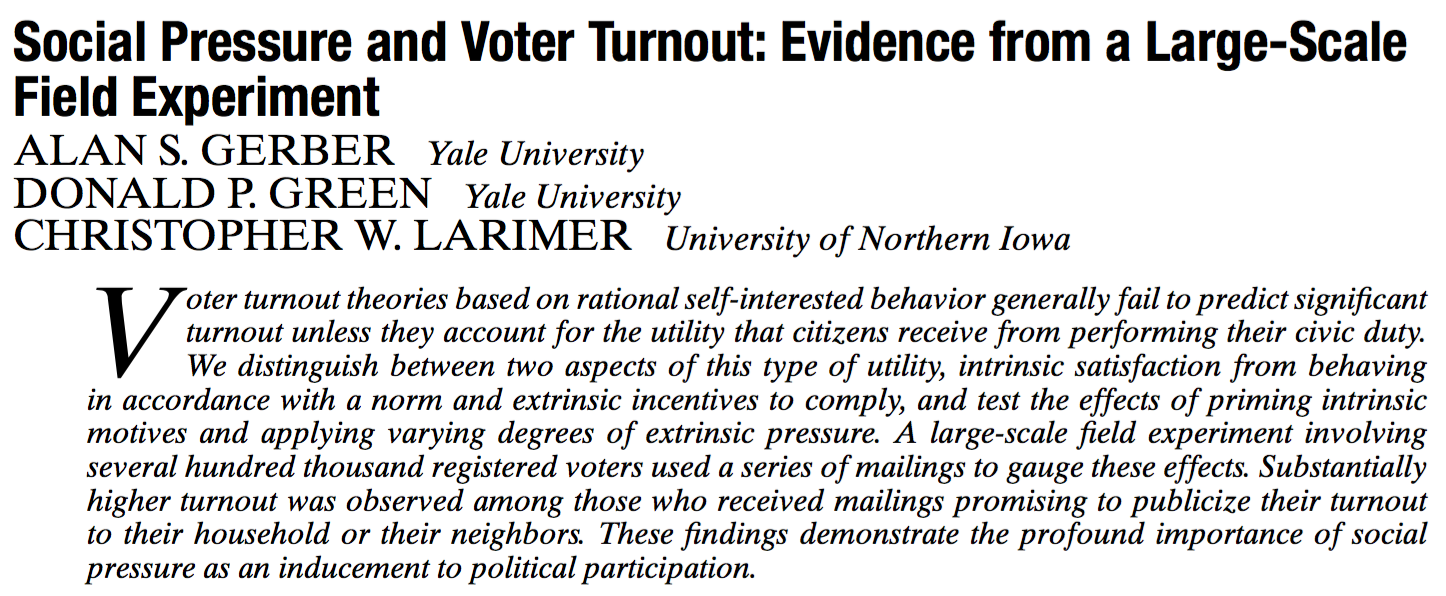
\includegraphics[width=4in]{abstractGGL}
\end{center}

}

\frame{
\frametitle{The Civic Duty Treatment}

\begin{center}

\includegraphics[width=4in]{CivicDutyGGL}
\end{center}

}

\frame{
\frametitle{The Hawthorne Treatment}

\begin{center}
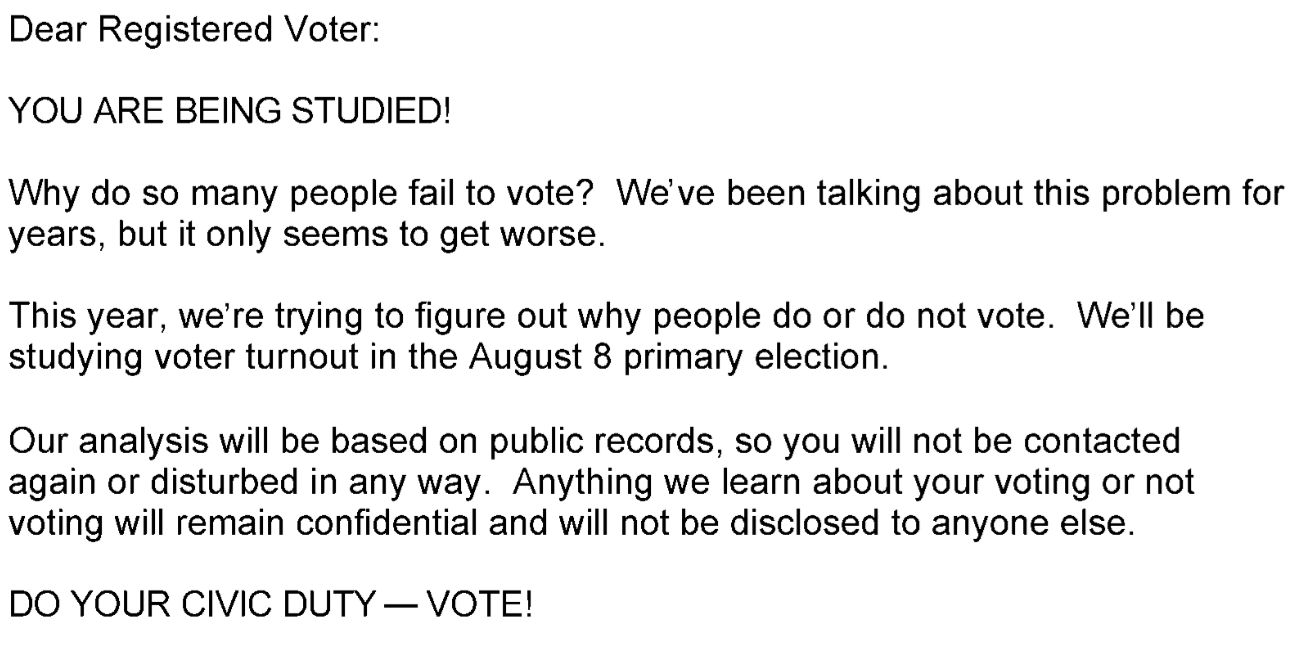
\includegraphics[width=4in]{HawthorneGGL}
\end{center}

}

\frame{
\frametitle{The Self Treatment}

\begin{center}
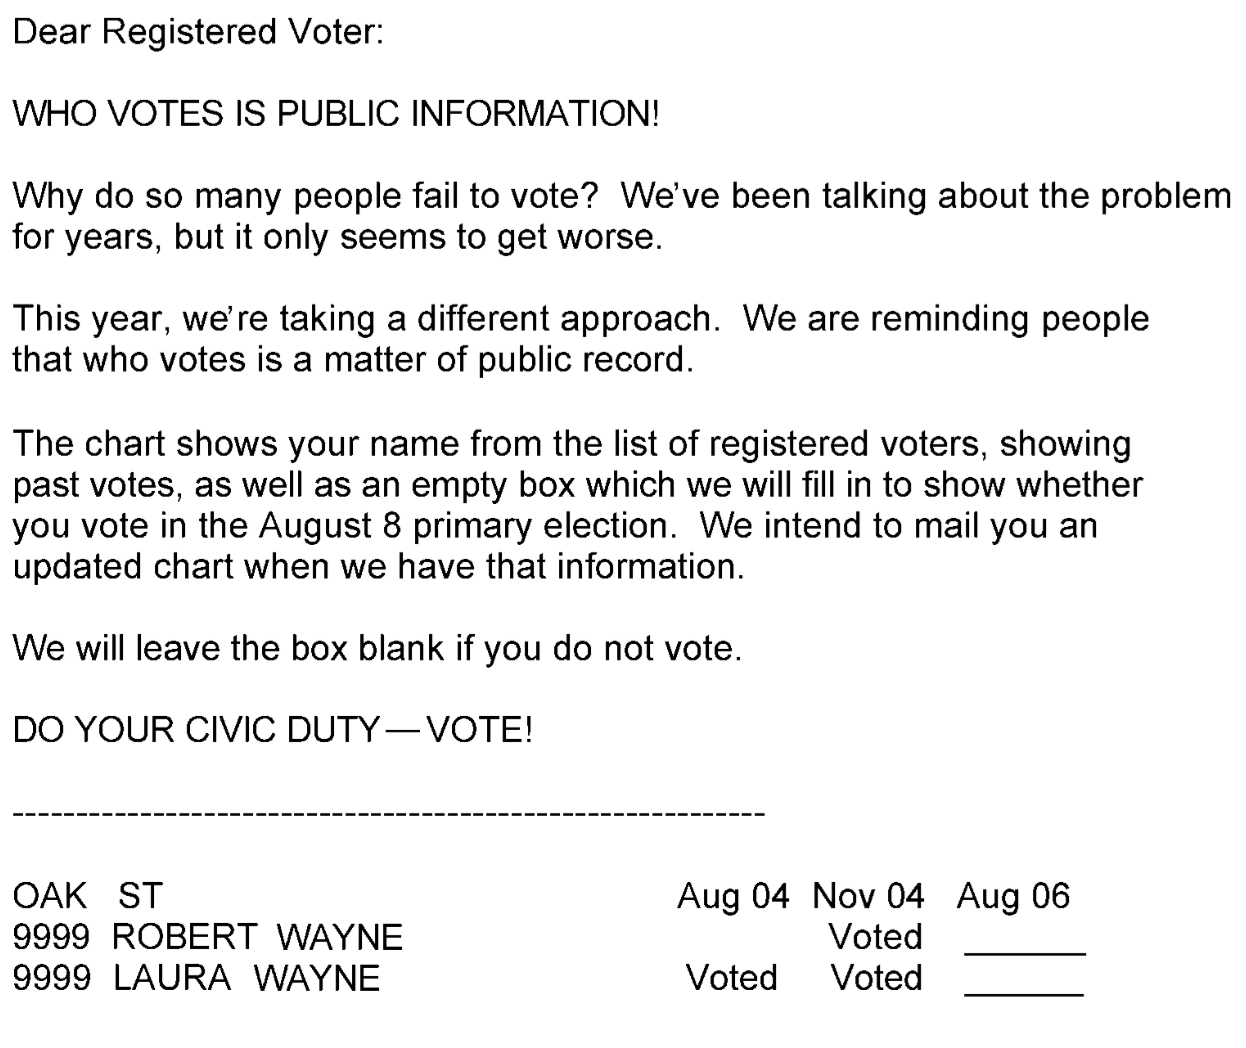
\includegraphics[width=3.5in]{SelfGGL}
\end{center}

}

\frame{
\frametitle{The Neighbors Treatment}

\begin{center}
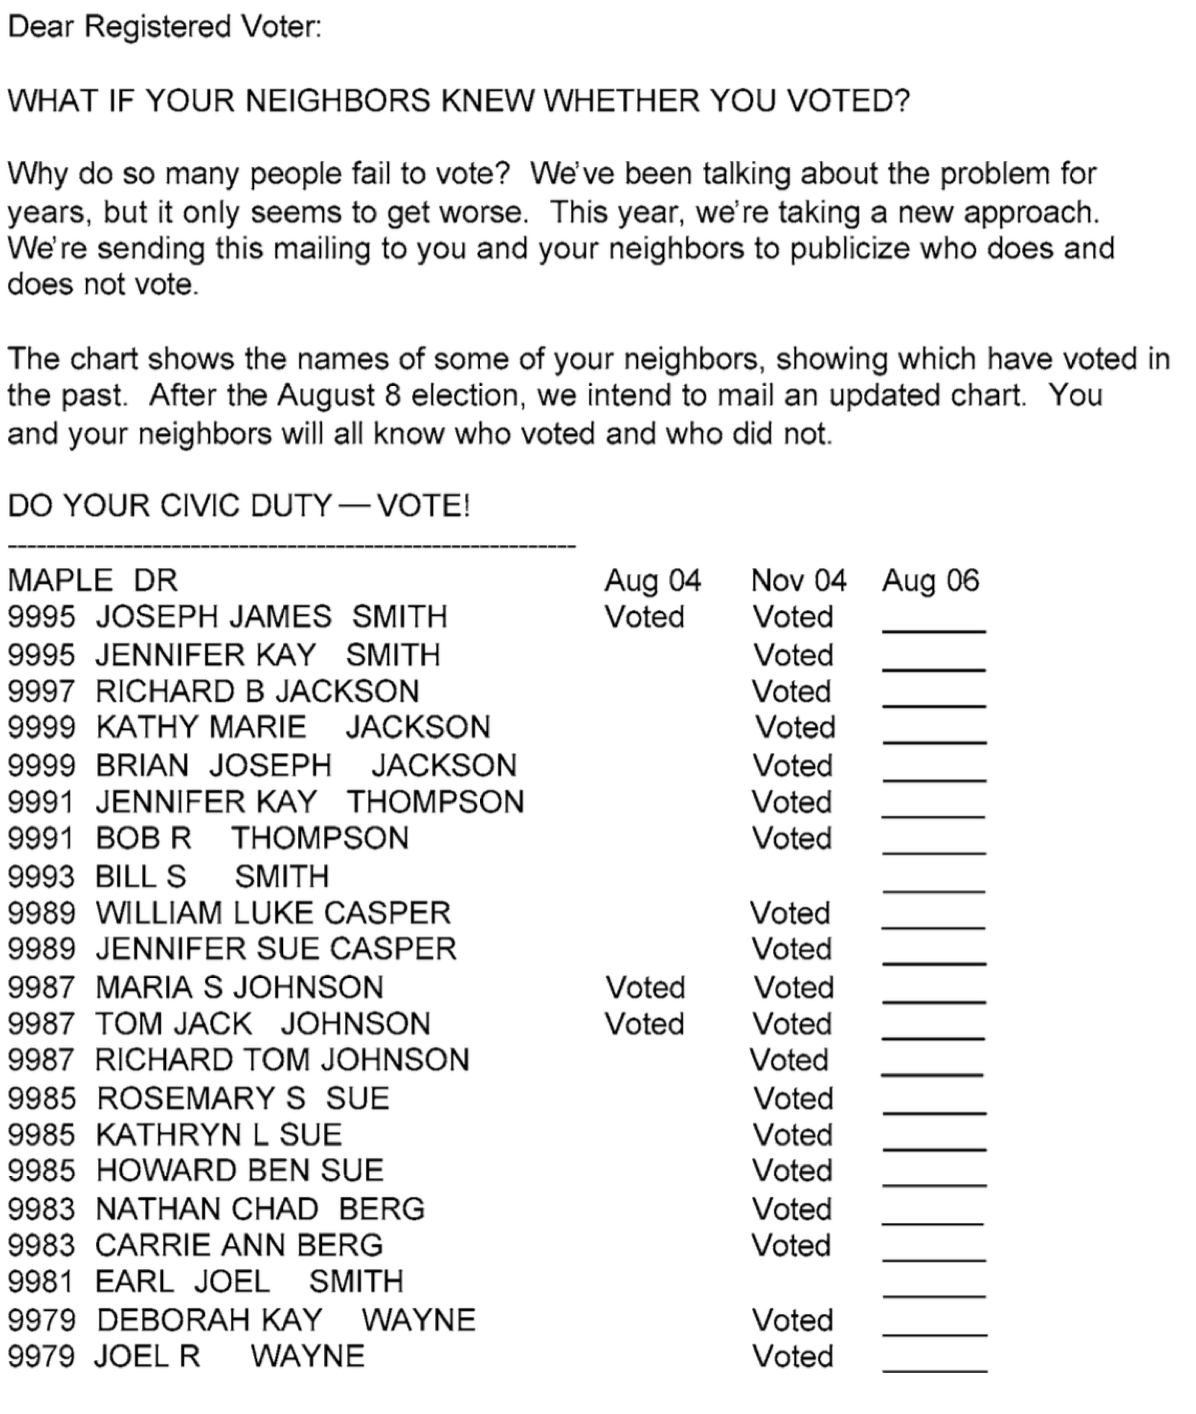
\includegraphics[width=3.5in]{NeighborsGGL}
\end{center}

}



\frame{
\frametitle{Balance on Pre-treatment Variables in the Gerber, Green, and Larimer Experiment}

\begin{center}
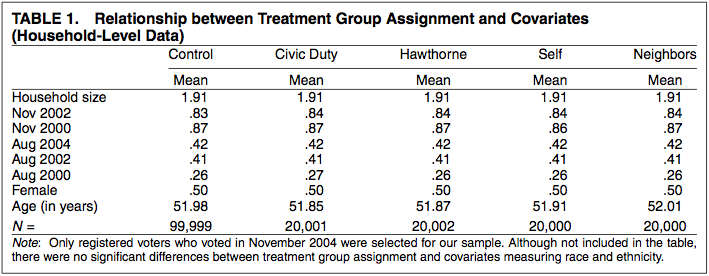
\includegraphics[width=4in]{GGL}
\end{center}

}


\frame{
\frametitle{Including Covariates in the Gerber, Green, and Larimer Experiment}

\begin{center}
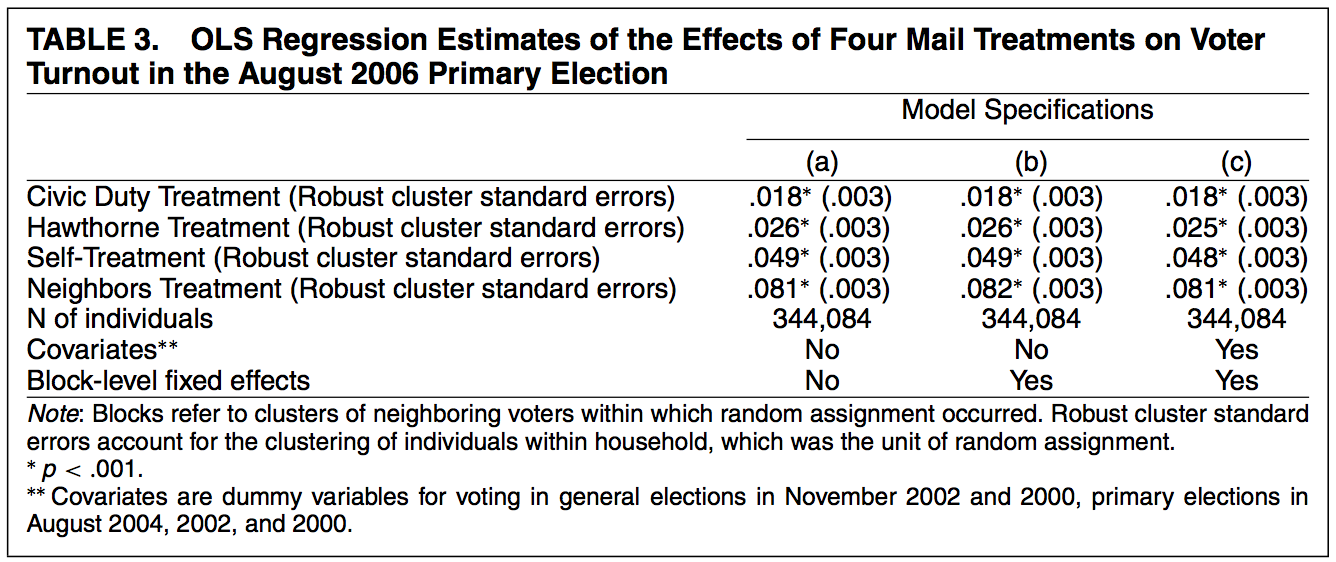
\includegraphics[width=4in]{GGL2}
\end{center}

}



\begin{frame}
\frametitle{FWL Theorem in Pictures}

Results: $$\hat{\beta}_{X}^{Y \sim X+Z} = \hat{\beta}_{r_{X\sim Z}}^{Y \sim r_{X\sim Z}}$$

$$\hat{\beta}_{X}^{Y \sim X+Z} = \hat{\beta}_{r_{X \sim Z}}^{r_{Y\sim Z} \sim r_{X\sim Z}}$$




\end{frame}


\begin{frame}[fragile]
\frametitle{Simulating Linear Model Data}

\begin{verbatim}
> n <- 10000
> set.seed(1234)
> z <- rnorm(n)
> x <- z + rnorm(n)
> y <- x + z + rnorm(n)
> cor(x,z)
[1] 0.7044271
\end{verbatim}

\end{frame}

\begin{frame}[fragile]
\frametitle{Linear Regression Output}

\begin{verbatim}
> lm(y ~ x)

Coefficients:
(Intercept)            x  
    0.01099      1.48301  

> lm(y ~ x + z)

Coefficients:
(Intercept)            x            z  
    0.00417      0.99901      0.98608 
\end{verbatim}

\end{frame}

\begin{frame}[fragile]
\frametitle{Added Variable ``Plot'' (Partial Regression ``Plot'')}

\begin{verbatim}
> r_yz <- residuals(lm(y ~ z))
> r_xz <- residuals(lm(x ~ z))
> r_yxz <- residuals(lm(y ~ x+z))
> lm(r_yz ~ r_xz)

Coefficients:
(Intercept)         r_xz  
 -3.619e-16    9.990e-01  

> range(r_yxz - residuals(lm(r_yz ~ r_xz)))
[1] -2.211564e-13  4.019007e-14
\end{verbatim}

\end{frame}


\begin{frame}[fragile]
\frametitle{Only $x$ residualized}

\begin{verbatim}
> lm(y ~ r_xz)

Coefficients:
(Intercept)         r_xz  
   0.008571     0.999006  

> range(r_yxz - residuals(lm(y ~ r_xz)))
[1] -7.209635  6.790846
\end{verbatim}

\end{frame}

\frame{
What if $x$ and $z$ are uncorrelated?

\bigskip

What if $x$ and $z$ perfectly correlated?

}

\frame{
What if $x$ and $z$ are uncorrelated?

\bigskip

$$\hat{\beta}_{X}^{Y \sim X} = \hat{\beta}_{X}^{Y \sim X + Z}$$

\ \ \ \ \ \ \ \ \ \ \ \ \ \ \ \ \ \ \ \ \ \ \ \ \ \ \ \ \ \ \ \ \ \ \ \ \ \ \ \ Why? (see whiteboard) 

\bigskip

What if $x$ and $z$ perfectly correlated?

}

\frame{
What if $x$ and $z$ are uncorrelated?

\bigskip

$$\hat{\beta}_{X}^{Y \sim X} = \hat{\beta}_{X}^{Y \sim X + Z}$$

\ \ \ \ \ \ \ \ \ \ \ \ \ \ \ \ \ \ \ \ \ \ \ \ \ \ \ \ \ \ \ \ \ \ \ \ \ \ \ \ Why? (see whiteboard) 

\bigskip

What if $x$ and $z$ perfectly correlated?

\ \ \ \ \ \ \ \ \ \ \ \ \ \ \ \ \ \ \ \ \ \ \ \ \ \ \ \ \ \ \ \ \ \ \ \ \ \ \ \ We can't fit a regression! 

}



\begin{frame}[fragile]
\frametitle{What if $x$ and $z$ are uncorrelated?}

\begin{verbatim}
> z <- rnorm(n)
> x <- rnorm(n) # no z
> cor(x,z)
[1] 0.01075281
> y <- x + z + rnorm(n)
> lm(y ~ x)
Coefficients:
(Intercept)            x  
    0.01027      1.00940  

> lm(y ~ x + z)

Coefficients:
(Intercept)            x            z  
    0.00417      0.99901      0.98509  
    \end{verbatim}

\end{frame}



\frame{
\frametitle{Summary}

\begin{itemize}
\item Additive linear multiple regression is a parsimonious summary of the relationship of multiple variables with an outcome, however care must be taken with the ``simple'' interpretation. 
\item Interactive linear multiple regression provides a more flexible summary but complicates the interpretation. However, sometimes we can average over the complications. 
\item Within additive models, the omitted variable formula and FWL theorem provide insight into the effect of controlling for an additional variable. Stable results can imply research credibility. 
\end{itemize}

}




%\frame{
%\frametitle{Summary}
%
%\begin{itemize}
%\item There are many possible descriptive questions with many variables and variables that take many values. 
%\item In this course we focus on means (possibly conditional), although variance and standard deviation are also concerns. 
%\item Conditioning requires modeling choices. In this course we use linear models (with and without interactions). 
%\end{itemize}
%
%}
%
%\frame{
%\frametitle{Next Week}
%
%Randomly Sampled Observations and Basic Probability
%
%\begin{itemize}
%\item Elementary Probability Theory
%\item Random Variables and Functions of Random Variables (Expectation, Variance, ...)
%\item Joint and Conditional Distributions
%\end{itemize}
%
%\vspace{.5cm}
%
%Things to do:
%\begin{itemize}
%\item first problem set
%\item the reading and the reading quiz
%\item annotations (if you have a question or want to respond to a question)
%\end{itemize}
%
%
%
%}



\end{document}












